\documentclass[reviewcopy]{elsart}
%\documentclass{elsart}
% Use the option doublespacing or reviewcopy to obtain double line spacing
% \documentclass[doublespacing]{elsart}
\usepackage{natbib}
\usepackage{endfloat}           % Float pics to the end
\usepackage{color}
\usepackage{url}
\usepackage{graphicx}
\usepackage{subfigure}
\usepackage{units}
\usepackage{amsmath}

\input{../cimis_acronyms} % CIMIS Acronyms

\begin{document}
%
\begin{frontmatter}
  \title{Daily reference evapotranspiration for California using
    satellite imagery and weather station measurement interpolation}
%
\author[calspace]{Quinn~Hart\corauthref{cor}}
\corauth[cor]{Corresponding author.}
\ead{qjhart@ucdavis.edu}
\author[calspace]{Marcela~Brugnach\thanksref{marcela}}
\ead{mbrugnac@usf.uos.de}
\author[cimis]{Bekele~Temesgen}
\ead{temesgen@water.ca.gov}
\author[calspace]{Carlos~Rueda}
\ead{carueda@ucdavis.edu}
\author[calspace]{Susan~Ustin}
\ead{slustin@ucdavis.edu}
\author[cimis]{Kent~Frame}
\ead{kframe@water.ca.gov}

\address[calspace]{CalSpace, University of California, Davis, Davis, CA, USA }

%\address[marcela]{Institute of Environmental Systems Research \\
%University of Osnabrueck  \\
%Germany }
\thanks[marcela]{Currently: Institute of Environmental Systems
  Research, University of Osnabrueck, Germany }

\address[cimis]{California Irrigation Management Information System
  (CIMIS), California Department of Water Resources, Sacramento, CA,
  USA }

\begin{abstract}
  Spatially distributed \ac{ET0} is calculated to produce daily
  \ac{ET0} maps for the State of California at high spatial
  resolution, $(\unit[2]{km})^2$.  Hourly \acs{NOAA} \acs{GOES} visible
  channel imager data are used to modify modeled radiation estimates.
  These are combined with interpolated \acf{CIMIS} weather station
  meteorological data to satisfy the Penman-Monteith \ac{ET0}
  equation.  Data have been acquired and \ac{ET0} estimated daily from
  February 2003 through April 2006.
\end{abstract}

\begin{keyword}
% keywords here, in the form: keyword \sep keyword
  evapotranspiration \sep Penman-Monteith equation \sep satellite
  imaging \sep remote sensing
% PACS codes here, in the form: \PACS code \sep code
% http://www.aip.org/pacs
\PACS 92.40.Zg \sep 92.40.Je \sep 42.68.Wt
\end{keyword}
\end{frontmatter}                                

% This format puts a special copyright style on the first page
%\thispagestyle{plain}

\begin{table}[htbp]
%  \hrule\vspace*{2pt}
  \centering
  \caption{Symbols used in this report}
  \label{tab:symbols}
  \begin{tabular}{l|l|l}
    Symbol & Description & Units \\
    \hline \hline
    \acs{ET} & \acl{ET} & \unitfrac{mm}{day} \\
    \acs{ET0} & \acl{ET0} & \unitfrac{mm}{day} \\
    \acs{Rn} & \acl{Rn} & \unitfrac{MJ}{m\ensuremath{^{2}}\,day} \\
    \acs{Rnl} & \acl{Rnl} & \unitfrac{MJ}{m\ensuremath{^{2}}\,day} \\
    \acs{Rs} &  \acl{Rs}   & \unitfrac{MJ}{m\ensuremath{^{2}}\,day} \\
    \acs{Rso} &  \acl{Rso}   & \unitfrac{MJ}{m\ensuremath{^{2}}\,day} \\
    \acs{G} & \acl{G}& \unitfrac{MJ}{m\ensuremath{^{2}}\,day} \\
    \acs{pa} & \acl{pa} & \unitfrac{kg}{m\ensuremath{^3}} \\
    \acs{cp} & \acl{cp} & \unitfrac{MJ}{kg \ensuremath{^\circ}{C}} \\
    \acs{ra} & \acl{ra} & \unitfrac{s}{m} \\
    \acs{rs} & \acl{rs} & \unitfrac{s}{m} \\
    \acs{Tm}  & \acl{Tm}  & \unit{\ensuremath{^\circ}C} \\
    \acs{Tn}  & \acl{Tn}  & \unit{\ensuremath{^\circ}C} \\
    \acs{Tx}  & \acl{Tx}  & \unit{\ensuremath{^\circ}C} \\
    \acs{dewp}  & \acl{dewp}  & \unit{\ensuremath{^\circ}C} \\
    \acs{U2} & \acl{U2}   & \unitfrac{m}{s} \\    
    \acs{RHx}& \acl{RHx}  & \unit{\%}\\
    \acs{ea} & \acl{ea}   & \unit{kPa} \\
    \acs{es} & \acl{es}   & \unit{kPa} \\
    \acs{psyc}& \acl{psyc}& \unitfrac{kPa}{\ensuremath{^\circ}C} \\
    \acs{vp}  & \acl{vp}  & \unitfrac{kPa}{\ensuremath{^\circ}C} \\
    \acs{K} &  \acl{K}   & \\
    \ensuremath{\sigma} & Stefan-Boltzmann constant = $4.903e^{-9}$ & \unitfrac{MJ}{m\ensuremath{^2}K\ensuremath{^4}\,day} \\
    \ensuremath{\alpha} & Albedo & \\
%%    \acs{em} & \acl{em} & \\
  \end{tabular}
\end{table}

\section{Introduction}

California experiences periodic water shortages from natural climate
variability, e.g., El Ni\~{n}o cycles, and is at risk for potential
longer-term extended droughts due to climate change. Winters with
below normal snowpack, either from low precipitation or early
snowmelt, cause low summer streamflow and inadequate water supplies
for agriculture and urban uses.  California agriculture is a \$25
billion/year economic sector and the economy is at risk without
efficient water management.  Improved monitoring can increase the
efficiency of water use and mitigate potential losses.

The \ac{CIMIS} program was successfully introduced by the California
Department of Water Resource and the University of California, Davis
in 1982, to help farmers, turf managers and other resource managers
develop water budgets that improve irrigation scheduling and limit
over-watering. The \ac{CIMIS} system is a repository of meteorological
data collected at over 130 computerized weather stations located at
key agricultural and municipal sites throughout California which
provide comprehensive, timely, weather data collected hourly and
daily.

This paper builds on the \ac{CIMIS} base by developing a methodology
to extend the weather station data to spatial daily \ac{ET0} maps of
California.  Daily reference \ac{ET0} maps for California are
calculated for a high spatial resolution $(\unit[2]{km})^2$ grid. We
developed daily statewide monitoring capability for estimating
reference evapotranspiration \ac{ET0} using the \ac{NOAA} \ac{GOES}
data and ground based weather data from the \ac{CIMIS} weather
stations.  Figure~\ref{fig:et0} shows an example \ac{ET0} map for
California.

\begin{figure}[htbp]
  \centering
  \resizebox{0.5\textwidth}{!}{\begin{picture}(0,0)%
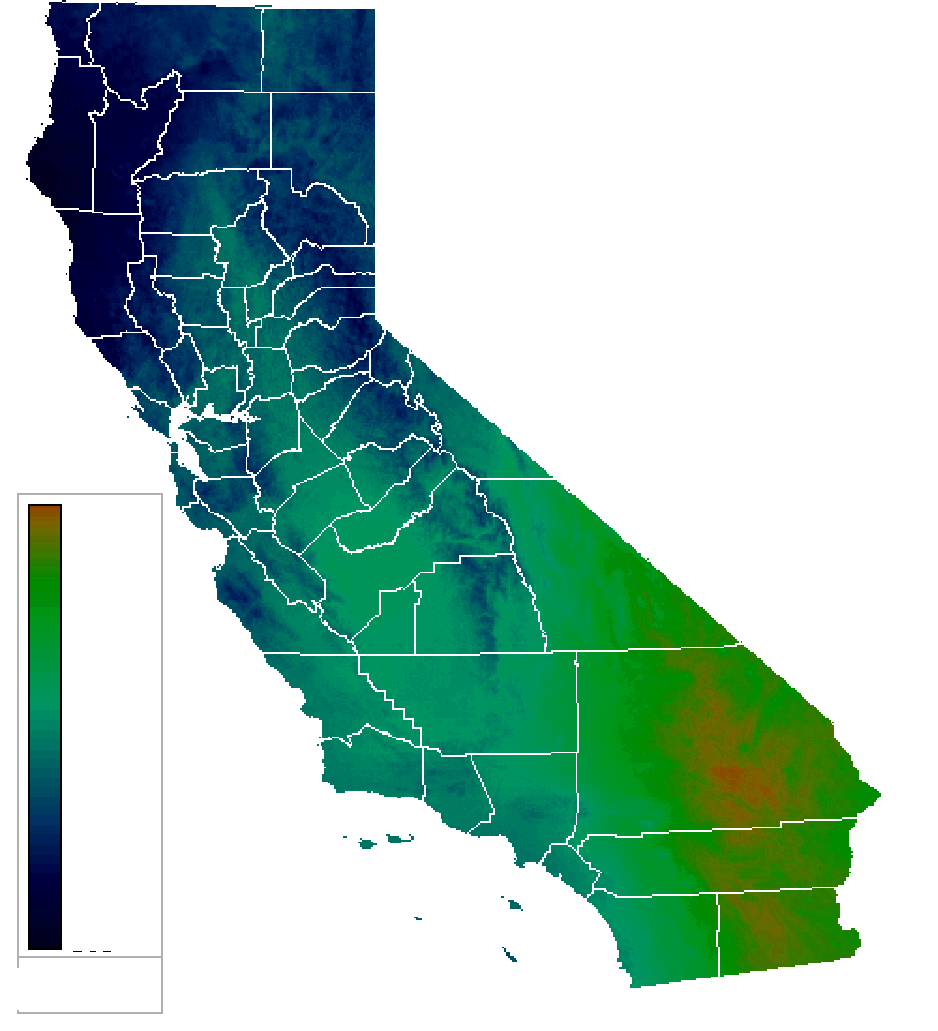
\includegraphics{2005/06/18/et0_fig.pdf}%
\end{picture}%
\setlength{\unitlength}{4144sp}%
%
\begingroup\makeatletter\ifx\SetFigFont\undefined%
\gdef\SetFigFont#1#2#3#4#5{%
  \reset@font\fontsize{#1}{#2pt}%
  \fontfamily{#3}\fontseries{#4}\fontshape{#5}%
  \selectfont}%
\fi\endgroup%
\begin{picture}(7143,7858)(1,-7019)
\put(586,-3166){\makebox(0,0)[lb]{\smash{{\SetFigFont{20}{24.0}{\rmdefault}{\mddefault}{\updefault}{\color[rgb]{0,0,0}9}%
}}}}
\put(586,-4021){\makebox(0,0)[lb]{\smash{{\SetFigFont{20}{24.0}{\rmdefault}{\mddefault}{\updefault}{\color[rgb]{0,0,0}7}%
}}}}
\put(586,-4831){\makebox(0,0)[lb]{\smash{{\SetFigFont{20}{24.0}{\rmdefault}{\mddefault}{\updefault}{\color[rgb]{0,0,0}5}%
}}}}
\put(586,-5596){\makebox(0,0)[lb]{\smash{{\SetFigFont{20}{24.0}{\rmdefault}{\mddefault}{\updefault}{\color[rgb]{0,0,0}3}%
}}}}
\put(586,-6316){\makebox(0,0)[lb]{\smash{{\SetFigFont{20}{24.0}{\rmdefault}{\mddefault}{\updefault}{\color[rgb]{0,0,0}1}%
}}}}
\put(226,-6766){\makebox(0,0)[lb]{\smash{{\SetFigFont{20}{24.0}{\rmdefault}{\mddefault}{\updefault}{\color[rgb]{0,0,0}mm}%
}}}}
\end{picture}%
}
  \caption{ \ac{ET0} estimations on 2005/06/18. The scale is in \unit{mm day$^-1$}.
}
  \label{fig:et0}
\end{figure}
    
% \section{Evapotranspiration}
% \label{sec:evapotranspiration}

% Evapotranspiration, \ac{ET}, is the combination of evaporation and
% transpiration processes. Evaporation is the free loss of water from
% soil and plant surfaces to the atmosphere.  Transpiration represents
% the plant mediated transfer of water, mainly through the stomata, to
% the atmosphere.  Evapotranspiration is controlled by physical factors,
% such as meteorological variables, soil characteristics, and the
% physiological characteristics of the vegetation such as plant type and
% biomass.

\ac{ET} is a measure of the water requirements for the healthy
functioning of a particular plant-soil-atmosphere system. By knowing
the water requirements of a particular system, a variety of water
issues, such as irrigation scheduling and design, landscape planning
and water transfer can be addressed.

% The Penman-Monteith equation for
% \ac{ET}~\citep{monteith65evapor-envir}, is defined as:

% \begin{equation}
%   \ac{ET} = \frac{\ac{vp} (\ac{Rn} - \ac{G}) +
%     \ac{pa}\ac{cp}\frac{(\ac{es} -
%       \ac{ea})}{\ac{ra}}}{\ac{vp} + \gamma (1 +
%     \frac{\ac{rs}}{\ac{ra}})} \label{eq:et}
% \end{equation}

% where the terms are defined in Table~\ref{tab:symbols}.  The \ac{ET}
% equation combines an energy balance with a simplified mass transfer
% model matching two resistances, the external or \ac{ra}, and the
% internal, or \ac{rs}.  Evapotranspiration is constrained by the
% available energy required to evaporate water. The control of
% environmental factors is expressed through the radiation budget, vapor
% pressure deficit and water vapor conductance.

By specifying standard crop parameters with a well irrigated
system, a standard \ac{ET0} can be determined that requires only
meteorological measurements.  A standardized \ac{ET0} separates
atmospheric drivers on \ac{ET} from crop specifics, and reduces the
need to develop more complex models for specific crop types and growth
stages.  Generally, field specific \acp{ET} are developed as simple
linear relationships to \ac{ET0}.

The \ac{ASCE} \ac{ASCE-ET} defines one standardized reference
evapotranspiration equation and two reference
surfaces~\citep{walter00stand-refer}.  The reference equation is:

\begin{equation}
  \ac{ET0} = \frac{0.408 \ac{vp} (\ac{Rn} - \ac{G}) +
    \ac{psyc}\frac{C_n}{T+273}(\ac{es} - \ac{ea})}{\ac{vp} + \ac{psyc} (1 +
    \frac{C_d}{\ac{U2}})} \label{eq:asce-et0}
\end{equation}

This paper uses the hypothetical short crop surface for \ac{ET0},
which resembles an extensive surface of green grass of uniform height,
actively growing with adequate water and a canopy completely shading
the ground.  The reference crop has an assumed height of
\unit[0.12]{m}, daily \ac{rs} of \unit[70]{sm\ensuremath{^{-1}}}, and
coefficients,$C_n = 900$ and $C_d = 0.34$.

The \ac{ASCE-ET} equation describes the control that
environmental factors, such as solar radiation, wind speed, air
temperature and humidity exert on \ac{ET0}. These factors influence
\ac{ET} either by providing the energy for vaporization or by
increasing efficiency in the removal of water vapor from the surface.

The following equations describe the parameters in the \ac{ET0}
equation in more detail:

\begin{align}
  \ac{ET0} &= \frac{0.408  \ac{vp}  (\ac{Rn} - \ac{G}) + \gamma \frac{900}{ \ac{Tm} + 273} \ac{U2} (\ac{es} - \ac{ea})}{\ac{vp} + \gamma  (1 + 0.34 \ac{U2})} \label{eq:et0} \\
  \ac{Rn} &= \ac{Rns} - \ac{Rnl} \label{eq:rn} \\
  \ac{Rns} &= (1 - \alpha) \ac{Rs} \label{eq:rns}\\
  \ac{Rs} &= \ac{K} \ac{Rso} \label{eq:rs}\\
  \ac{Rnl} &= (1.35\frac{\ac{Rs}}{R_{so}}-0.35)(0.34-0.14\sqrt{ea})\sigma\frac{\ac{Tn}^4+\ac{Tx}^4}{2} \label{eq:rnl} \\
  \ac{vp}    &= \frac{4099  \ac{ea}}{ (\ac{Tm} + 237.3)^2} \label{eq:delta} \\
  \ac{psyc}&= 0.665\text{e-3}(101.3{\frac{293-0.0065z}{293}}^{5.26}) \\
  \ac{Tm}   &= \frac{\ac{Tn} + \ac{Tx}}{2} \label{eq:Tm}\\
  \ac{es}   &= \frac{0.6108}{2}  \left(\exp\left(\frac{17.27 \ac{Tn}}{\ac{Tn} + 237.3}\right) + \exp\left(\frac{17.27 \ac{Tx}}{\ac{Tx}+237.3}\right)\right) \label{eq:es}\\
  \ac{ea}  &= 0.6108 \exp\left(\frac{17.27 \ac{dewp}}{\ac{dewp} + 237.3}\right)\label{eq:eadewp}
\end{align}

$\ac{Rn}-\ac{G}$ represents the supply of energy available to vaporize
water.  For daily calculations, net radiation, \ac{Rn}, is dominant
and soil heat flux density, \ac{G}, is assumed to be negligible.
\ac{Rn} is calculated as the difference between the incoming net
shortwave radiation, \ac{Rns} and the outgoing net longwave radiation,
\ac{Rnl}, (Eq.~\ref{eq:rn}).  \ac{Rns} represents the portion of
\ac{Rs} that is not reflected (Eq.~\ref{eq:rs}), where \ac{Rs}, is the
amount of incoming solar radiation that reaches the earth surface
after accounting for the effects of absorption, scattering and
reflection of the atmosphere.  \ac{Rs} is modeled as
a fraction of \ac{Rso}, where \ac{K} is determined from \ac{GOES}
satellite data, more fully described in Section~\ref{sec:radiation}.
The reference crop has an albedo of 0.23.  Net longwave radiation,
\ac{Rnl} represents the exchange of radiation between the crop surface
and the atmosphere and clouds (Eq.~\ref{eq:rnl}).

In the \ac{ET0} equation, the water content of the air is represented
with $(\ac{es} - \ac{ea})$ expressing the vapor pressure deficit.
Saturation vapor pressure, \ac{es}, is computed as the mean between
saturation vapor pressure at maximum air temperature and saturation
vapor pressure at minimum air temperature (Eq.~\ref{eq:es}).  The
actual vapor pressure, \ac{ea} is calculated as a function of dew
point temperature (Eq.~\ref{eq:eadewp}).  The slope of the vapor
pressure-temperature curve is \ac{vp} (Eq.~\ref{eq:delta}) and
\ac{psyc} is the psychrometric constant.  \ac{Tm} is the mean air
temperature (Eq.~\ref{eq:Tm}).

\section{\ac{ET0} Parameter Estimation}

Calculating \ac{ET0} requires meteorological data including; air
temperature, incoming solar radiation, average daily wind speed and
dew point temperature. Solar radiation is derived from models coupled
with \ac{GOES} satellite imagery for cloud cover estimation.
Temperatures, wind speed and dew point are derived by interpolating
point data from the network of \ac{CIMIS} weather stations.

For spatial estimates of \ac{ET0}, the parameters need to be
calculated for every pixel in a gridded surface of California.
Figure~\ref{fig:process} shows an overview of all steps for
calculating statewide \ac{ET0}.  These steps include procedures for
spatially interpolating \ac{CIMIS} data as well as processing
\ac{GOES} image data to predict the \acl{K} and the resultant
\acl{Rs}.  All processing steps are performed using existing or
created modules in the \ac{GRASS}~\citep{GRASS_GIS_software,
  neteler04open-sourc-gis} \ac{GIS} application.

\begin{figure*}[htbp]
  \centering
  \resizebox{1\textwidth}{!}{\begin{picture}(0,0)%
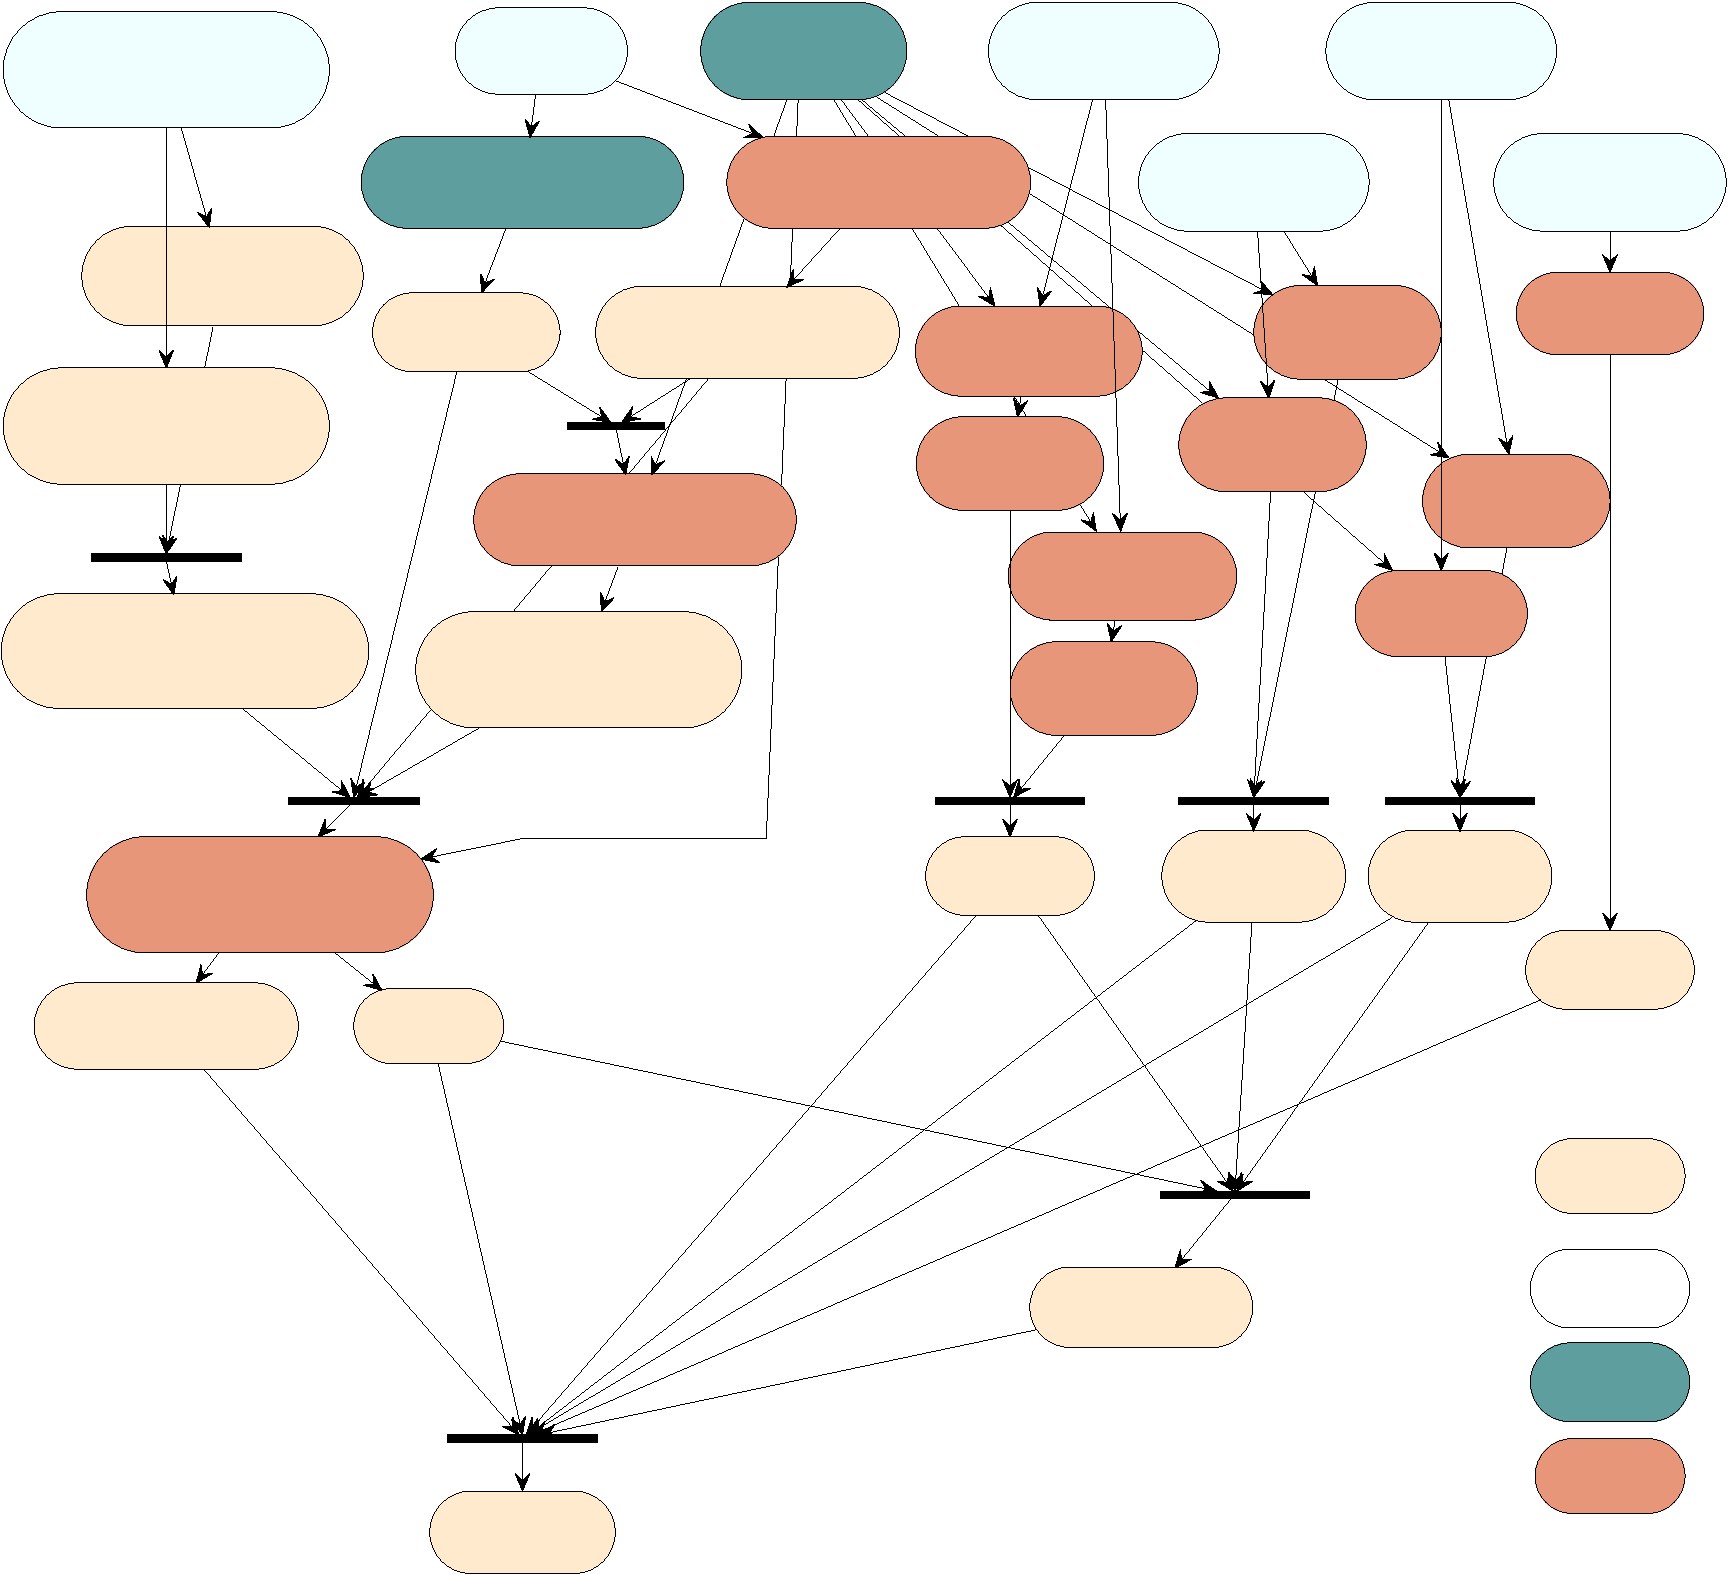
\includegraphics{figs/process_fig.pdf}%
\end{picture}%
\setlength{\unitlength}{3947sp}%
%
\begingroup\makeatletter\ifx\SetFigFont\undefined%
\gdef\SetFigFont#1#2#3#4#5{%
  \reset@font\fontsize{#1}{#2pt}%
  \fontfamily{#3}\fontseries{#4}\fontshape{#5}%
  \selectfont}%
\fi\endgroup%
\begin{picture}(13819,12594)(921,-11953)
\put(5101,-11701){\makebox(0,0)[b]{\smash{{\SetFigFont{12}{14.4}{\ttdefault}{\mddefault}{\updefault}{\color[rgb]{0,0,0}\ETo}%
}}}}
\put(4351,-7651){\makebox(0,0)[b]{\smash{{\SetFigFont{12}{14.4}{\ttdefault}{\mddefault}{\updefault}{\color[rgb]{0,0,0}\K}%
}}}}
\put(2251,-7651){\makebox(0,0)[b]{\smash{{\SetFigFont{12}{14.4}{\ttdefault}{\mddefault}{\updefault}{\color[rgb]{0,0,0}\Rs}%
}}}}
\put(10051,-9901){\makebox(0,0)[b]{\smash{{\SetFigFont{12}{14.4}{\ttdefault}{\mddefault}{\updefault}{\color[rgb]{0,0,0}\Rnl}%
}}}}
\put(9001,-6451){\makebox(0,0)[b]{\smash{{\SetFigFont{12}{14.4}{\ttdefault}{\mddefault}{\updefault}{\color[rgb]{0,0,0}\ea}%
}}}}
\put(10951,-6451){\makebox(0,0)[b]{\smash{{\SetFigFont{12}{14.4}{\ttdefault}{\mddefault}{\updefault}{\color[rgb]{0,0,0}\Tx}%
}}}}
\put(12601,-6451){\makebox(0,0)[b]{\smash{{\SetFigFont{12}{14.4}{\ttdefault}{\mddefault}{\updefault}{\color[rgb]{0,0,0}\Tn}%
}}}}
\put(11101,-3009){\makebox(0,0)[b]{\smash{{\SetFigFont{12}{14.4}{\ttdefault}{\mddefault}{\updefault}{\color[rgb]{0,0,0}\Tx (TG)}%
}}}}
\put(11701,-2109){\makebox(0,0)[b]{\smash{{\SetFigFont{12}{14.4}{\ttdefault}{\mddefault}{\updefault}{\color[rgb]{0,0,0}\Tx (RST)}%
}}}}
\put(12451,-4359){\makebox(0,0)[b]{\smash{{\SetFigFont{12}{14.4}{\ttdefault}{\mddefault}{\updefault}{\color[rgb]{0,0,0}\Tn (TG)}%
}}}}
\put(13051,-3459){\makebox(0,0)[b]{\smash{{\SetFigFont{12}{14.4}{\ttdefault}{\mddefault}{\updefault}{\color[rgb]{0,0,0}\Tn (RST)}%
}}}}
\put(10951,-781){\makebox(0,0)[b]{\smash{{\SetFigFont{12}{14.4}{\ttdefault}{\mddefault}{\updefault}{\color[rgb]{0,0,0}\Tx}%
}}}}
\put(10951,-1029){\makebox(0,0)[b]{\smash{{\SetFigFont{12}{14.4}{\ttdefault}{\mddefault}{\updefault}{\color[rgb]{0,0,0}Point Data}%
}}}}
\put(7351,254){\makebox(0,0)[b]{\smash{{\SetFigFont{12}{14.4}{\ttdefault}{\mddefault}{\updefault}{\color[rgb]{0,0,0}Digital}%
}}}}
\put(7351, 21){\makebox(0,0)[b]{\smash{{\SetFigFont{12}{14.4}{\ttdefault}{\mddefault}{\updefault}{\color[rgb]{0,0,0}Elevation}%
}}}}
\put(12451,269){\makebox(0,0)[b]{\smash{{\SetFigFont{12}{14.4}{\ttdefault}{\mddefault}{\updefault}{\color[rgb]{0,0,0}\Tn}%
}}}}
\put(12451, 21){\makebox(0,0)[b]{\smash{{\SetFigFont{12}{14.4}{\ttdefault}{\mddefault}{\updefault}{\color[rgb]{0,0,0}Point data}%
}}}}
\put(9151,-2266){\makebox(0,0)[b]{\smash{{\SetFigFont{12}{14.4}{\ttdefault}{\mddefault}{\updefault}{\color[rgb]{0,0,0}\dewp (TG)}%
}}}}
\put(9901,-4066){\makebox(0,0)[b]{\smash{{\SetFigFont{12}{14.4}{\ttdefault}{\mddefault}{\updefault}{\color[rgb]{0,0,0}\dewp (RST)}%
}}}}
\put(9751,254){\makebox(0,0)[b]{\smash{{\SetFigFont{12}{14.4}{\ttdefault}{\mddefault}{\updefault}{\color[rgb]{0,0,0}\dewp}%
}}}}
\put(9751, 21){\makebox(0,0)[b]{\smash{{\SetFigFont{12}{14.4}{\ttdefault}{\mddefault}{\updefault}{\color[rgb]{0,0,0}Point Data}%
}}}}
\put(9001,-3159){\makebox(0,0)[b]{\smash{{\SetFigFont{12}{14.4}{\ttdefault}{\mddefault}{\updefault}{\color[rgb]{0,0,0}\acs{ea} (TG)}%
}}}}
\put(9751,-4959){\makebox(0,0)[b]{\smash{{\SetFigFont{12}{14.4}{\ttdefault}{\mddefault}{\updefault}{\color[rgb]{0,0,0}\ea (RST)}%
}}}}
\put(4651,-2116){\makebox(0,0)[b]{\smash{{\SetFigFont{12}{14.4}{\ttdefault}{\mddefault}{\updefault}{\color[rgb]{0,0,0}Turbidity}%
}}}}
\put(6901,-1981){\makebox(0,0)[b]{\smash{{\SetFigFont{12}{14.4}{\ttdefault}{\mddefault}{\updefault}{\color[rgb]{0,0,0}Sunrise/Sunset}%
}}}}
\put(6901,-2243){\makebox(0,0)[b]{\smash{{\SetFigFont{12}{14.4}{\ttdefault}{\mddefault}{\updefault}{\color[rgb]{0,0,0}Hour Angle}%
}}}}
\put(5551,-4553){\makebox(0,0)[b]{\smash{{\SetFigFont{12}{14.4}{\ttdefault}{\mddefault}{\updefault}{\color[rgb]{0,0,0}Clear Sky}%
}}}}
\put(5551,-4809){\makebox(0,0)[b]{\smash{{\SetFigFont{12}{14.4}{\ttdefault}{\mddefault}{\updefault}{\color[rgb]{0,0,0}Direct,Diffuse}%
}}}}
\put(5551,-5049){\makebox(0,0)[b]{\smash{{\SetFigFont{12}{14.4}{\ttdefault}{\mddefault}{\updefault}{\color[rgb]{0,0,0}radiance}%
}}}}
\put(7951,-773){\makebox(0,0)[b]{\smash{{\SetFigFont{12}{14.4}{\ttdefault}{\mddefault}{\updefault}{\color[rgb]{0,0,0}Solar Position}%
}}}}
\put(7951,-1021){\makebox(0,0)[b]{\smash{{\SetFigFont{12}{14.4}{\ttdefault}{\mddefault}{\updefault}{\color[rgb]{0,0,0}Model}%
}}}}
\put(2401,-4381){\makebox(0,0)[b]{\smash{{\SetFigFont{12}{14.4}{\ttdefault}{\mddefault}{\updefault}{\color[rgb]{0,0,0}kXXXX}%
}}}}
\put(2401,-4666){\makebox(0,0)[b]{\smash{{\SetFigFont{12}{14.4}{\ttdefault}{\mddefault}{\updefault}{\color[rgb]{0,0,0}Hourly Estimates}%
}}}}
\put(2401,-4891){\makebox(0,0)[b]{\smash{{\SetFigFont{12}{14.4}{\ttdefault}{\mddefault}{\updefault}{\color[rgb]{0,0,0}of Cloud Cover}%
}}}}
\put(5251,261){\makebox(0,0)[b]{\smash{{\SetFigFont{12}{14.4}{\ttdefault}{\mddefault}{\updefault}{\color[rgb]{0,0,0}Today's}%
}}}}
\put(5251, 37){\makebox(0,0)[b]{\smash{{\SetFigFont{12}{14.4}{\ttdefault}{\mddefault}{\updefault}{\color[rgb]{0,0,0}Date}%
}}}}
\put(5101,-796){\makebox(0,0)[b]{\smash{{\SetFigFont{12}{14.4}{\ttdefault}{\mddefault}{\updefault}{\color[rgb]{0,0,0}Global Turbidty}%
}}}}
\put(5101,-1021){\makebox(0,0)[b]{\smash{{\SetFigFont{12}{14.4}{\ttdefault}{\mddefault}{\updefault}{\color[rgb]{0,0,0}Database}%
}}}}
\put(6001,-3473){\makebox(0,0)[b]{\smash{{\SetFigFont{12}{14.4}{\ttdefault}{\mddefault}{\updefault}{\color[rgb]{0,0,0}Solar Radiation}%
}}}}
\put(6001,-3721){\makebox(0,0)[b]{\smash{{\SetFigFont{12}{14.4}{\ttdefault}{\mddefault}{\updefault}{\color[rgb]{0,0,0}Model}%
}}}}
\put(2251,-2573){\makebox(0,0)[b]{\smash{{\SetFigFont{12}{14.4}{\ttdefault}{\mddefault}{\updefault}{\color[rgb]{0,0,0}maxXXXX}%
}}}}
\put(2251,-2866){\makebox(0,0)[b]{\smash{{\SetFigFont{12}{14.4}{\ttdefault}{\mddefault}{\updefault}{\color[rgb]{0,0,0}Hourly Visible}%
}}}}
\put(2251,-3099){\makebox(0,0)[b]{\smash{{\SetFigFont{12}{14.4}{\ttdefault}{\mddefault}{\updefault}{\color[rgb]{0,0,0}Maximum Values}%
}}}}
\put(2251,261){\makebox(0,0)[b]{\smash{{\SetFigFont{12}{14.4}{\ttdefault}{\mddefault}{\updefault}{\color[rgb]{0,0,0}visXXXX}%
}}}}
\put(2251,-16){\makebox(0,0)[b]{\smash{{\SetFigFont{12}{14.4}{\ttdefault}{\mddefault}{\updefault}{\color[rgb]{0,0,0}Hourly Visible}%
}}}}
\put(2251,-256){\makebox(0,0)[b]{\smash{{\SetFigFont{12}{14.4}{\ttdefault}{\mddefault}{\updefault}{\color[rgb]{0,0,0}GOES Images}%
}}}}
\put(3001,-6353){\makebox(0,0)[b]{\smash{{\SetFigFont{12}{14.4}{\ttdefault}{\mddefault}{\updefault}{\color[rgb]{0,0,0}Hourly Solar}%
}}}}
\put(3001,-6593){\makebox(0,0)[b]{\smash{{\SetFigFont{12}{14.4}{\ttdefault}{\mddefault}{\updefault}{\color[rgb]{0,0,0}Radiation Model}%
}}}}
\put(3001,-6871){\makebox(0,0)[b]{\smash{{\SetFigFont{12}{14.4}{\ttdefault}{\mddefault}{\updefault}{\color[rgb]{0,0,0}and Integration}%
}}}}
\put(13801,-7201){\makebox(0,0)[b]{\smash{{\SetFigFont{12}{14.4}{\ttdefault}{\mddefault}{\updefault}{\color[rgb]{0,0,0}\U}%
}}}}
\put(13801,-781){\makebox(0,0)[b]{\smash{{\SetFigFont{12}{14.4}{\ttdefault}{\mddefault}{\updefault}{\color[rgb]{0,0,0}\U}%
}}}}
\put(13801,-1029){\makebox(0,0)[b]{\smash{{\SetFigFont{12}{14.4}{\ttdefault}{\mddefault}{\updefault}{\color[rgb]{0,0,0}Point Data}%
}}}}
\put(13801,-1816){\makebox(0,0)[b]{\smash{{\SetFigFont{12}{14.4}{\ttdefault}{\mddefault}{\updefault}{\color[rgb]{0,0,0}2D}%
}}}}
\put(13801,-2101){\makebox(0,0)[b]{\smash{{\SetFigFont{12}{14.4}{\ttdefault}{\mddefault}{\updefault}{\color[rgb]{0,0,0}Slpine}%
}}}}
\put(13801,-8829){\makebox(0,0)[b]{\smash{{\SetFigFont{12}{14.4}{\ttdefault}{\mddefault}{\updefault}{\color[rgb]{0,0,0}rasters}%
}}}}
\put(13801,-9646){\makebox(0,0)[b]{\smash{{\SetFigFont{12}{14.4}{\ttdefault}{\mddefault}{\updefault}{\color[rgb]{0,0,0}Daily}%
}}}}
\put(13801,-9886){\makebox(0,0)[b]{\smash{{\SetFigFont{12}{14.4}{\ttdefault}{\mddefault}{\updefault}{\color[rgb]{0,0,0}Inputs}%
}}}}
\put(13801,-10373){\makebox(0,0)[b]{\smash{{\SetFigFont{12}{14.4}{\ttdefault}{\mddefault}{\updefault}{\color[rgb]{0,0,0}Static}%
}}}}
\put(13801,-10613){\makebox(0,0)[b]{\smash{{\SetFigFont{12}{14.4}{\ttdefault}{\mddefault}{\updefault}{\color[rgb]{0,0,0}Data}%
}}}}
\put(13801,-11236){\makebox(0,0)[b]{\smash{{\SetFigFont{12}{14.4}{\ttdefault}{\mddefault}{\updefault}{\color[rgb]{0,0,0}Models}%
}}}}
\put(2701,-1531){\makebox(0,0)[b]{\smash{{\SetFigFont{12}{14.4}{\ttdefault}{\mddefault}{\updefault}{\color[rgb]{0,0,0}pXXXX}%
}}}}
\put(2701,-1793){\makebox(0,0)[b]{\smash{{\SetFigFont{12}{14.4}{\ttdefault}{\mddefault}{\updefault}{\color[rgb]{0,0,0}Hourly Albedo}%
}}}}
\end{picture}%
}
  \caption{Processing steps for generating \ac{ET0}. The left side shows
    the integration of hourly \ac{GOES} imagery to estimate radiation
    parameters.  The right side shows weather station interpolations
    usually with two procedures.}
\label{fig:process}
\end{figure*}

Figure~\ref{fig:process}, shows two separate methods were used to
calculate temperature related parameters, discussed in
Section~\ref{sec:ground-stat-interp}.  This small ensemble of
estimates gives a measure of potential errors in the estimates, and
are used in a sensitivity analysis of the results, discussed in
Section~\ref{sec:meas-uncert}.

\subsection{Ground Station Data Interpolation}
\label{sec:ground-stat-interp}

Maximum air temperature, \ac{Tx}, minimum air temperature, \ac{Tn},
dew point, \ac{dewp}, and average wind speed, \ac{U2}, are derived by
spatially interpolating point data from the \ac{CIMIS} network. These
weather stations are spatially distributed as shown in
Figure~\ref{fig:stations}.  Areas such as California's central valley
have a dense distribution of stations, but mountainous, urban, and
desert regions are less represented.  This distribution results from
the design to inform California's agricultural irrigation practices.
For various reasons, not all stations report data daily; on average it
is possible to use data from about 120 stations.
Figure~\ref{fig:stations} groups stations by elevation with higher
stations having larger symbols.  Figure~\ref{fig:stations} also
identifies three small transects used to validate temperature lapse
rates.

\begin{figure}[htbp]
  \centering
    \resizebox{.5\textwidth}{!}{\begin{picture}(0,0)%
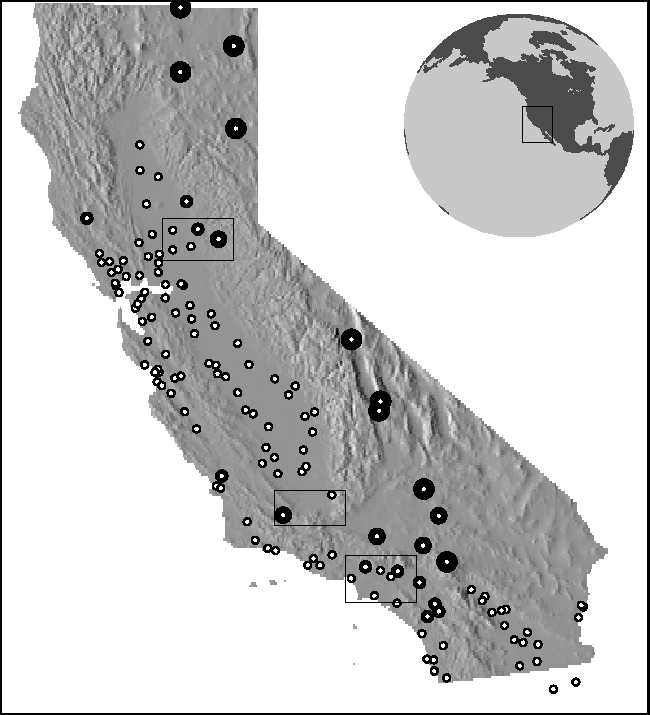
\includegraphics{figs/stations_fig.pdf}%
\end{picture}%
\setlength{\unitlength}{4144sp}%
%
\begingroup\makeatletter\ifx\SetFigFont\undefined%
\gdef\SetFigFont#1#2#3#4#5{%
  \reset@font\fontsize{#1}{#2pt}%
  \fontfamily{#3}\fontseries{#4}\fontshape{#5}%
  \selectfont}%
\fi\endgroup%
\begin{picture}(4948,5445)(22,-4606)
\put(2611,-2806){\makebox(0,0)[lb]{\smash{{\SetFigFont{12}{14.4}{\familydefault}{\mddefault}{\updefault}{\color[rgb]{0,0,0}South Valley}%
}}}}
\put(2071,-3976){\makebox(0,0)[lb]{\smash{{\SetFigFont{12}{14.4}{\familydefault}{\mddefault}{\updefault}{\color[rgb]{0,0,0}South Coast}%
}}}}
\put(2026,-871){\makebox(0,0)[lb]{\smash{{\SetFigFont{12}{14.4}{\familydefault}{\mddefault}{\updefault}{\color[rgb]{0,0,0}Sacramento}%
}}}}
\end{picture}%
}

    \caption{\ac{CIMIS} weather stations.  Larger symbols imply higher elevations.}
  \label{fig:stations}
\end{figure}

Spatial interpolation generates surfaces of continuous fields from
data collected at discrete locations. Interpolation methods are built
on assumptions that attributes are continuous over space and values
close together are more similar than those farther apart.

Several interpolation methods were investigated.  Criteria for method
selection included accuracy of results, code availability, and
computational efficiency.  Multiple interpolations created a small
ensemble of predictions that allowed for an estimation of errors.
After investigating several methods, we used \ac{RST} and \ac{TG}
interpolations.

The \ac{TG}, sometimes identified as
DayMet~\citep{thornton.ea:97:daymet} method refers to an interpolation
method that generates daily surfaces of temperature, humidity and
other variables over large regions of complex terrain.  The method
applies the spatial convolution of a Gaussian filter with a set of
observations.  The weight $W_{t,\alpha}(r)$ given to an observation
with a radial distance $r$ from the center of the filter is given by
$W_{t,\alpha}(r) = \exp(-(r/t)^2\alpha) - \exp(-\alpha)$.  The
parameter $t$ determines a truncation distance such that the weight is
zero if $r>t$. The parameter $\alpha$ adjusts the shape of the filter.

On a daily basis, we determine these parameters by exhaustively
searching the parameter space and selecting the values that minimize
the estimation error using the standard leave-one-out cross-validation
methodology.  The \ac{TG} method estimates the truncation radius via
an iterative algorithm such that it is decreased for regions with high
observation density and increased otherwise.  Elevation data are
included in the method as a post-correction step. In the case of
temperature, this is performed by weighted least-square regression.

Although the \ac{TG} method is applied as an inverse-distance algorithm,
the Gaussian function does not force the resultant surface to pass
through the observations, thus allowing for smoother surfaces.

\ac{RST}~\citep{mitasova.ea:95:rstgrass,neteler04open-sourc-gis} is a
method that simulates passing a flexible plate close to the known data
points while minimizing the energy to bend the plate.  Two parameters
drive the shape of the interpolation.  The tension parameter tunes the
plate from stiff to flexible.  Low tension (stiff) plates are
smoother, but can miss high gradient changes.  High tension (flexible)
plates are less smooth and allow higher gradient changes about
individual points.  Tension also controls the influence of neighboring
points.  Lower tension gives points influence over longer distances.

The smoothing parameter controls how much the fitted surface can
deviate from the measured point values. Since the spatial
interpolation assigns one value for each (\unit[2]{km})$^2$ pixel,
variation of the \ac{RST} from the measured points is allowed.

Both 2-dimensional and 3-dimensional splines with elevation were used.
2-D \acp{RST} interpolations along with lapse rate normalization were
made for temperature estimations.  Wind speed estimations used 3-D
splines. Parameter values were selected through cross-validation
exercises in conjunction with visual inspection and were kept constant
for all estimates.

One example of how the location of \ac{CIMIS} stations is not
representative of California is the distribution of stations as a
function of elevation.  Figure~\ref{fig:elevation} shows the
difference in the distribution and range of the elevation, comparing
the \ac{CIMIS} stations and California as a whole.  The station
elevations under-represent the higher elevations in California.
Because of this, extrapolating temperature measurements from CIMIS
stations to regions with differing elevations is error prone.

\begin{figure}
  \centering
  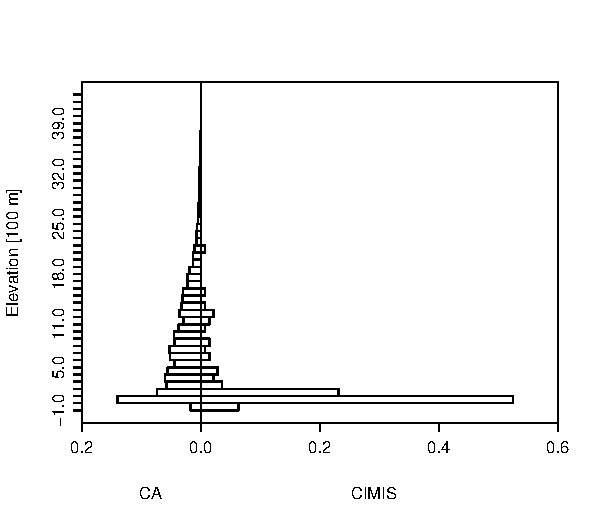
\includegraphics[width=.5\textwidth]{Z.pdf}
  \caption{Histograms of elevations for California from a
    $(\unit[2]{km})^2$ digital elevation model and \ac{CIMIS}
    stations.  }
\label{fig:elevation}
\end{figure}

The \ac{RST} interpolation uses a simple lapse rate to normalize the
temperatures from all stations to a standard elevation.  The
measurements were normalized to sea level using a standard lapse rate
of \unitfrac[5]{\ensuremath{^\circ}C}{km}.  A 2-D spline interpolation
was fit to the normalized data.  The parameters to the \ac{RST}, were
chosen with low tension and high smoothness resulting in a smooth
interpolation over the normalized data.  The resulting values were
then re-corrected by lapse rate along with elevation data for the
state.  Figure~\ref{fig:rst} shows an example for temperatures
calculated using this method.

\begin{figure}[htbp]
  \centering
  \mbox{
    \subfigure[Normalized]{
      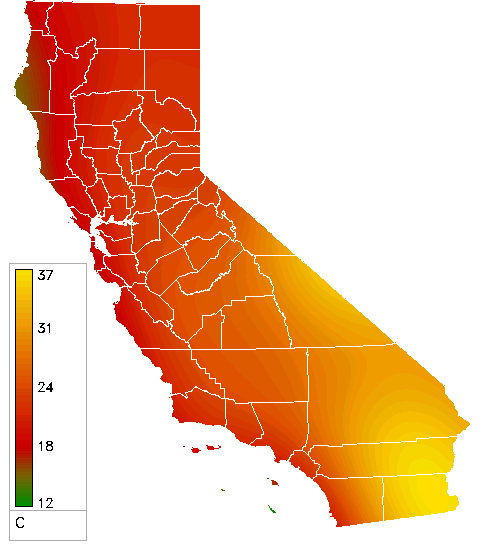
\includegraphics[width=0.5\textwidth]{2005/06/18/nd_max_at_lr5_t10_s0_03.png}
    } \quad
    \subfigure[Elevation Corrected]{
      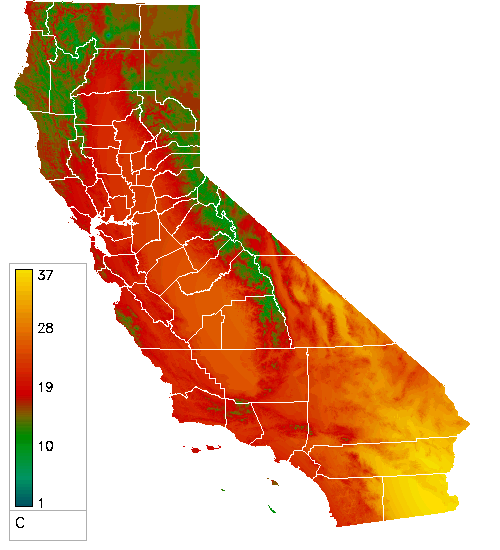
\includegraphics[width=0.5\textwidth]{2005/06/18/d_max_at_ns.png}
    }
  }
  \caption{
%
    \acf{RST} interpolations from air temperatures on 2005/06/18
    normalized to sea level, and the air temperature estimates after correcting
    for elevation.  The method predicts gradual changes in the
    normalized temperature, while maintaining strong elevation
    dependence of the temperature values.
%
  }
  \label{fig:rst}
\end{figure}

A lapse rate of \unitfrac[5]{\ensuremath{^\circ}C}{km} was chosen for
all temperature interpolations, \ac{Tx},\ac{Tn}, and \ac{dewp}.  An
examination of measured lapse rates between close stations, shows
lapse rates for California vary widely.  Figure~\ref{fig:stations}
shows three regions, labeled Sacramento, South Valley, and South
Coast, with some moderate elevation differences between proximate
stations.  To test the lapse rate within these regions, the difference
in temperature versus the difference in elevation was calculated for
all pairs of stations within each region, for each day in the three
year time window.  Figure~\ref{fig:lapse-rate} shows these
relationships and the calculated lapse rates for each region and
temperature interpolation.  The lapse rates vary widely between
regions, with only \ac{dewp} showing any statewide stability.

\begin{figure}
  \centering
  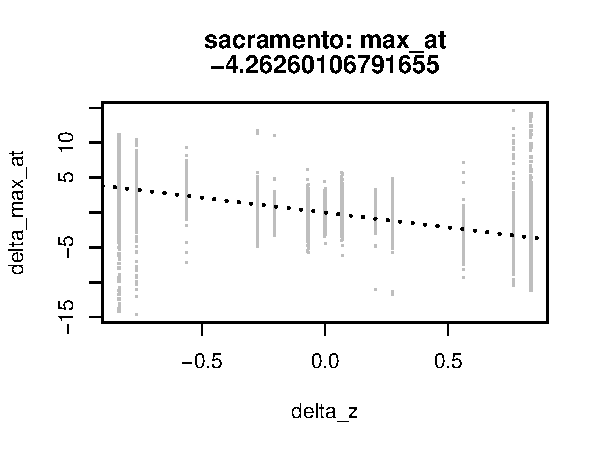
\includegraphics[width=0.3\textwidth]{lapse_rate/sacramento_max_at}
  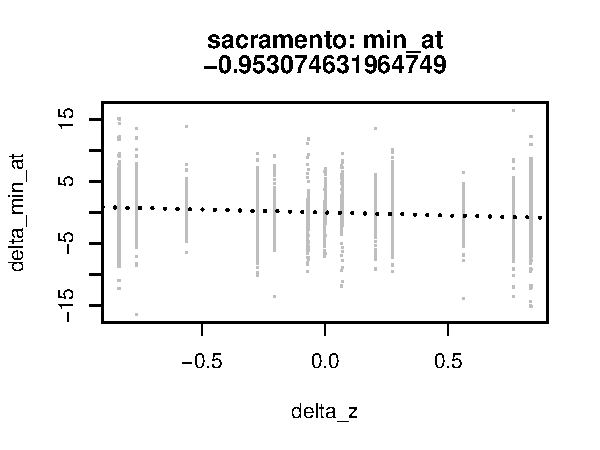
\includegraphics[width=0.3\textwidth]{lapse_rate/sacramento_min_at} 
  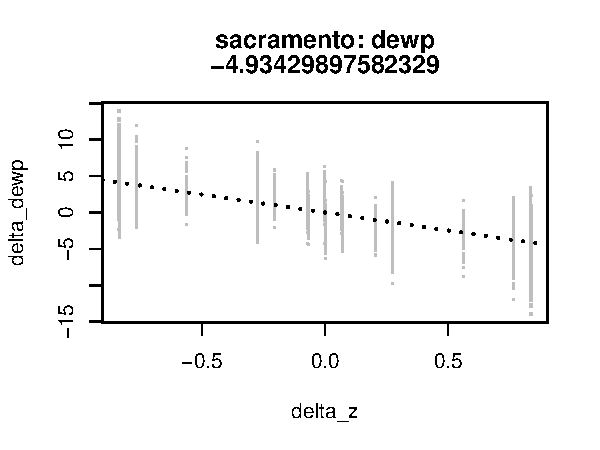
\includegraphics[width=0.3\textwidth]{lapse_rate/sacramento_dewp}

  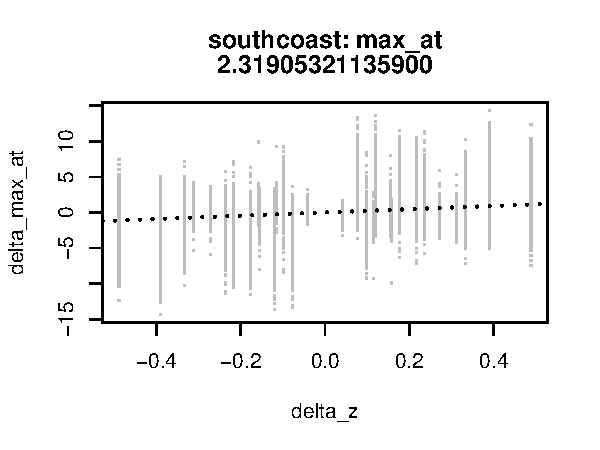
\includegraphics[width=0.3\textwidth]{lapse_rate/southcoast_max_at}
  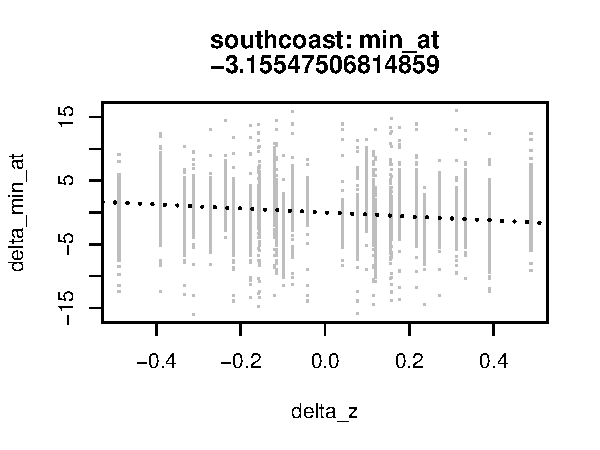
\includegraphics[width=0.3\textwidth]{lapse_rate/southcoast_min_at} 
  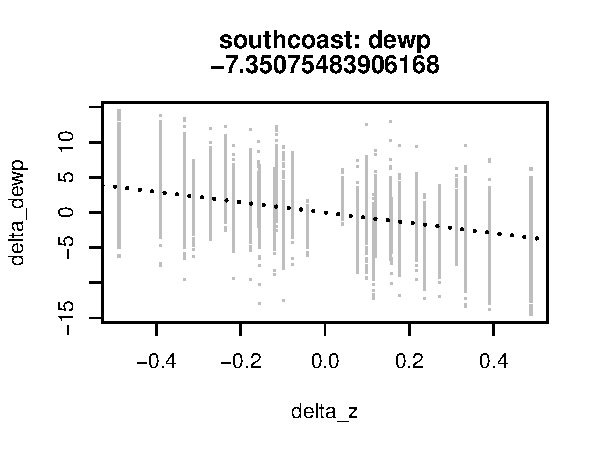
\includegraphics[width=0.3\textwidth]{lapse_rate/southcoast_dewp}

  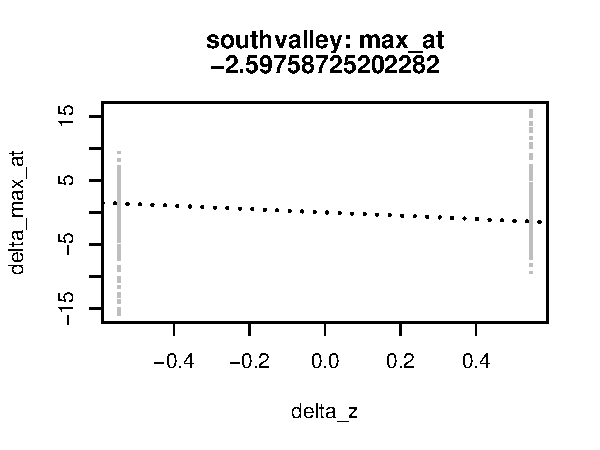
\includegraphics[width=0.3\textwidth]{lapse_rate/southvalley_max_at}
  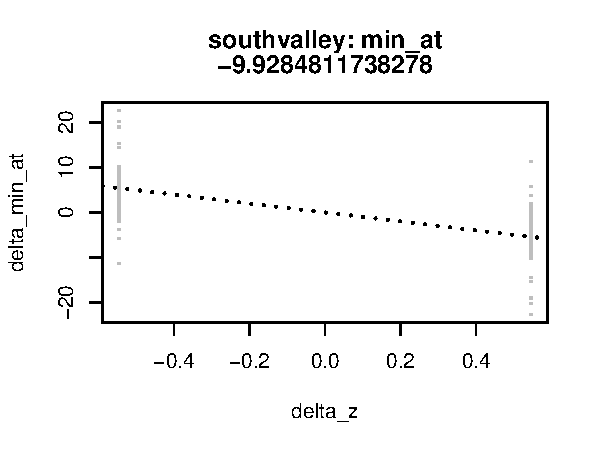
\includegraphics[width=0.3\textwidth]{lapse_rate/southvalley_min_at} 
  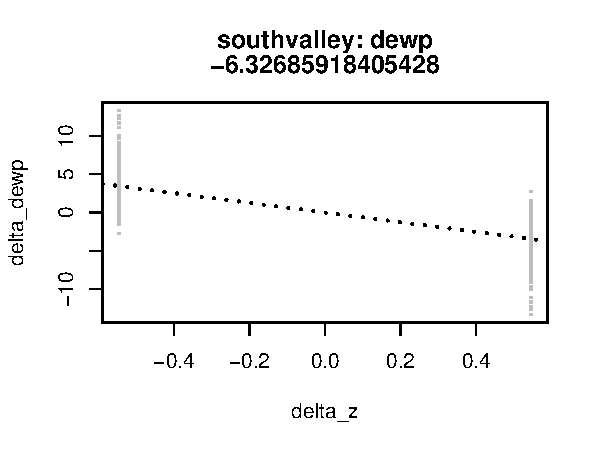
\includegraphics[width=0.3\textwidth]{lapse_rate/southvalley_dewp}
  \caption{Lapse rate measurements for three regions of California, for
\ac{Tx},\ac{Tn} and \ac{dewp}.
}
\label{fig:lapse-rate}
\end{figure}

Including seasonal differences compounds this confusion.
Table~\ref{tab:lapse_rate} shows lapse rates for these regions
averaged at monthly intervals.  In addition to regional differences,
time-dependant changes in lapse rate are apparent.  While it is fairly
easy to explain aspects of these results (for example, the diminishing
effect of maritime influences in the South Coast region causing an
inversion of lapse rates moving inland with higher elevations) it is
clear that simple interpolations over a complex landscape can be only
partially successful.

\begin{table}
  \centering
  \caption{Average monthly surface temperature lapse rate measurements $[\unitfrac{\ensuremath{^\circ}C}{km}]$ for various California transects.
  }
\begin{tabular}{c | c c c | c c c | c c c }
& \multicolumn{3}{c|}{South Coast} & \multicolumn{3}{c|}{South Valley} & \multicolumn{3}{c}{Sacramento} \\
\raisebox{1.5ex}{Month} & \ac{Tx} & \ac{Tn} & \ac{dewp} & \ac{Tx} & \ac{Tn}  &\ac{dewp} & \ac{Tx} & \ac{Tn} & \ac{dewp} \\ \hline \hline
Jan& -3.34& -3.81& -9.44& 3.25& -7.29& -7.66& 0.20& -1.93& -4.93\\
Feb& -3.13& -3.68& -10.22& -3.93& -7.50& -6.48& -4.50& -2.29& -5.62\\
Mar& 0.46& -3.94& -7.58& -4.73& -10.39& -6.14& -5.54& -2.49& -5.49\\
Apr& -0.46& -3.97& -6.42& -4.67& -10.18& -5.59& -6.50& -2.84& -3.83\\
May& 4.15& -3.09& -6.52& -3.79& -10.69& -5.65& -6.48& -2.43& -3.58\\
Jun& 6.63& -5.31& -3.76& -3.63& -12.83& -5.09& -5.47& -1.27& -3.33\\
Jul& 10.36& -2.38& -4.63& -2.91& -13.02& -6.46& -3.53& 2.67& -4.94\\
Aug& 9.99& -2.02& -6.04& -3.23& -12.51& -5.45& -3.09& 2.38& -6.50\\
Sep& 6.22& -0.80& -7.30& -3.17& -11.39& -5.39& -4.08& 0.81& -6.97\\
Oct& 1.56& -1.68& -5.74& -3.53& -8.34& -6.69& -4.68& -0.33& -5.27\\
Nov& -2.20& -3.64& -9.45& -0.94& -6.87& -8.38& -2.64& -0.55& -4.56\\
Dec& -3.05& -3.23& -11.06& 1.62& -5.71& -8.43& -2.33& -1.74& -4.28\\

\end{tabular}
\label{tab:lapse_rate}
\end{table}

Final temperature estimates were generated by averaging the
results of \ac{TG} and \ac{RST} interpolations.  Figure~\ref{fig:T}
shows a comparison of the two methods for a single day.

\begin{figure}[htbp]
  \centering
  \mbox{
    \subfigure[2005/06/18 \ac{TG}]{
      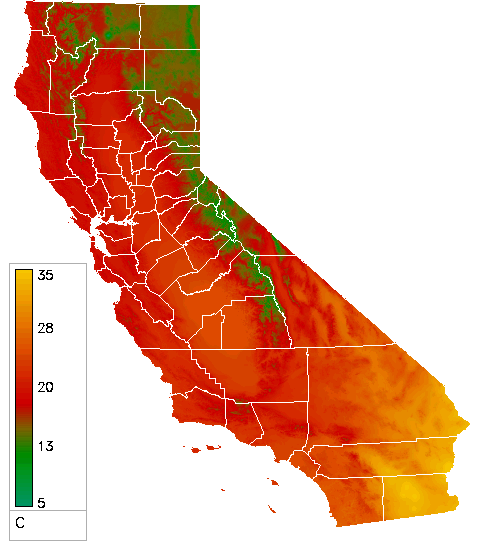
\includegraphics[width=.5\textwidth]{2005/06/18/d_max_at_dme.png}
    }\quad
    \subfigure[2005/06/18 Spline]{
      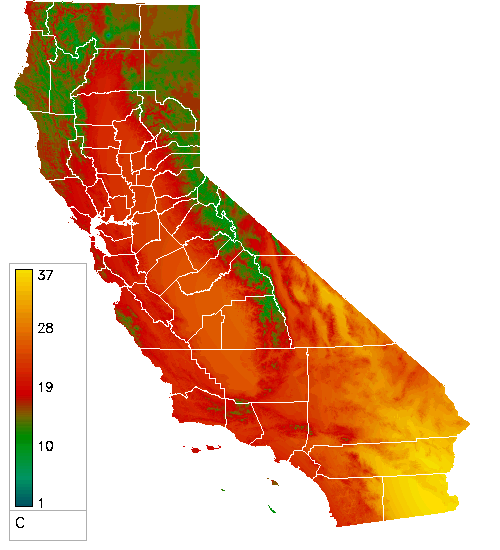
\includegraphics[width=.5\textwidth]{2005/06/18/d_max_at_ns.png}
    }
  }
   \caption{
%
     Example of temperature interpolation
     comparing the \ac{TG} method and \ac{RST} 
     for one day, 2005/06/18.
%
   }
  \label{fig:T}
% %\vspace*{12pt}\hrule
\end{figure}

% The actual vapor pressure, \ac{ea}, and saturation vapor pressure,
% \ac{es}, (Eq.~\ref{eq:es}), are used to estimate the vapor pressure
% deficit of the air. This deficit represents the gradient of water
% vapor between the evaporating surface and the air and constitutes one
% of the determinant drivers for the aerodynamic component of
% evapotranspiration.  \ac{ea} is also used as a correction in estimating
% longwave radiation (Eq~\ref{eq:rnl}).  \ac{ea} is calculated from the
% interpolated values of \ac{dewp}.

Average daily wind speed measured at \unit[2]{m} height above the
surface is used to compute the aerodynamic resistance, which
represents a resistance to diffusion that air above the vegetative
surface imposes on \ac{ET}. Average wind speed maps were generated
using 3D \ac{RST}.  Figure~\ref{fig:ws} shows some example wind speed
interpolations.  For these estimates, more flexible surfaces were fit.
High winds reported from single stations cause anomalous effects
in the interpolation around those points.  Another problem with wind
speed interpolations is that only the speed and not wind
direction is included in the interpolation model.

\begin{figure}[htbp]
  \centering
  \mbox{
    \subfigure[2005/06/18]{
      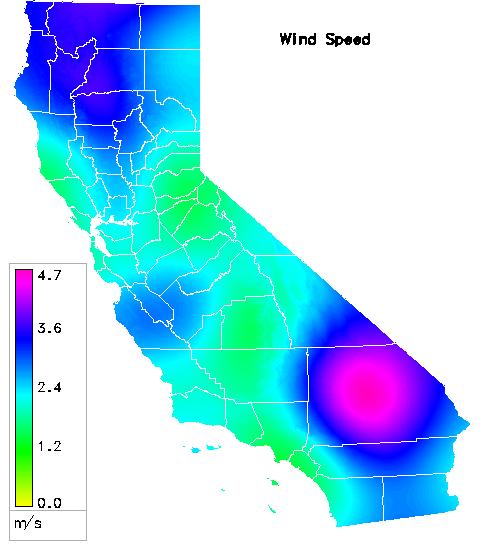
\includegraphics[width=.5\textwidth]{2005/06/18/U2.png}
    }\quad
    \subfigure[2005/12/21]{
      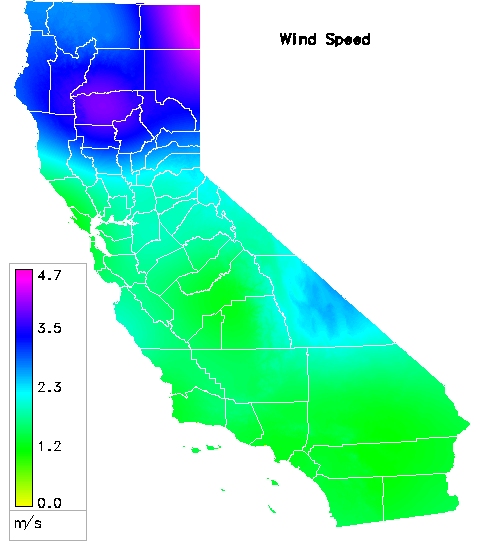
\includegraphics[width=.5\textwidth]{2005/12/21/U2.png}
    }
  }
  \caption{
%
    Two typical wind speed interpolations, for a
    calm and a windy day.
%
  }
  \label{fig:ws}
%\vspace*{12pt}\hrule
\end{figure}

\subsection{Radiation Models}
\label{sec:radiation}

Radiative inputs to the \ac{ASCE-ET} equation include the energy terms;
\ac{Rs} and \ac{Rnl}.  Solar radiation can be measured directly or
modeled. Longwave radiation is primarily a function of surface
temperature, but is also affected by the daily average cloud cover and
water vapor which affect the emissivity.

\subsubsection{Solar Radiation, \ac{Rs}}

Solar radiation is a linear term in the \ac{ET0} equation and in most
cases in California is the driving factor in its calculation.
Therefore it is important to measure this parameter accurately.
\ac{CIMIS} stations measure solar radiation directly, but this
parameter cannot be reliably interpolated spatially, since it is
dependant on the daily cloud cover, which does not interpolate well
from station data points.

The method for the calculation of \ac{Rs} combines model predictions
of clear sky radiation with hourly estimates of cloud cover using
\ac{GOES} visible channel imager data.  This method for estimating
solar radiation is independent of measurements at the \ac{CIMIS}
stations.  The clear sky solar radiation model used is
Heliosat-II~\citep{rigol.ea:00:on-clear,lefer.ea:02:descr-of}.

For each location in California, the sunrise and sunset times are
calculated each day.  Within the sunlit period, \ac{GOES} data are
available for each hour, as shown in Figure~\ref{fig:radiation}.  The
solar zenith angle for each hour are shown with solid lines.
From each of these hourly \ac{GOES} images, a clear sky factor is
calculated (Section~\ref{sec:cloud-brightn-clear}).  This factor is
assumed constant over the intervals of time/sun angle shown with
dotted lines.  Clear sky radiation is calculated for each of these
intervals.  The clear sky radiation and clear sky factor are used to
predict the actual radiation for each interval.  Finally, the
contributions from all intervals are summed for the daily estimate of
solar radiation.

\begin{figure}[htbp]
  \centering
  \resizebox{0.5\textwidth}{!}{\begin{picture}(0,0)%
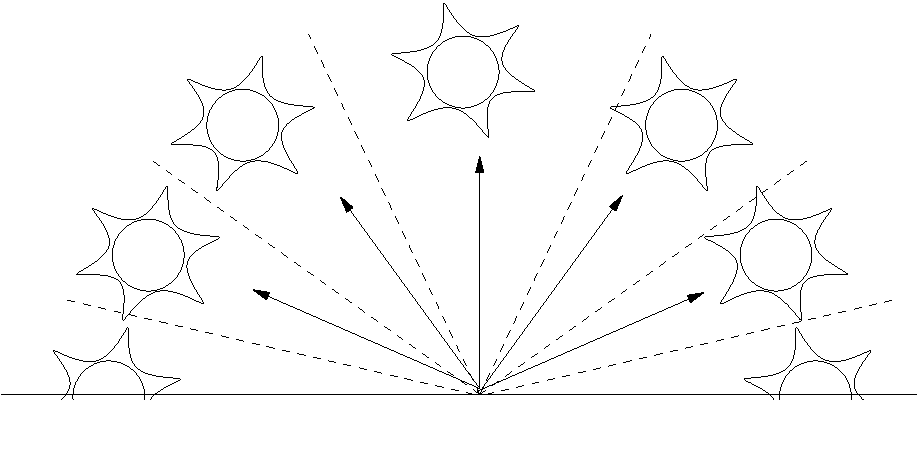
\includegraphics{insolation_fig.pdf}%
\end{picture}%
\setlength{\unitlength}{4144sp}%
%
\begingroup\makeatletter\ifx\SetFigFont\undefined%
\gdef\SetFigFont#1#2#3#4#5{%
  \reset@font\fontsize{#1}{#2pt}%
  \fontfamily{#3}\fontseries{#4}\fontshape{#5}%
  \selectfont}%
\fi\endgroup%
\begin{picture}(6999,3548)(1069,-3223)
\end{picture}%
}
  \caption{
%
    Solar radiation calculations are performed on zenith intervals, using hourly cloud cover estimates. 
%
  }
  \label{fig:radiation}
\end{figure}

The Heliosat-II model uses an analytical integration over solar angles
and it is simple to change the frequency of the \ac{GOES} cloud cover
estimates.  Missing cloud cover estimates, caused by lost \ac{GOES}
images, are handled by extending the intervals adjacent to the missing
times.  The analytical integration assigns appropriate weights to the
remaining cloud cover estimates.

Atmospheric transmission in the Heliosat-II model combines aspects of
aerosols, relative humidity, ozone, and molecular scattering into a
single parameter, the Linke turbidity, which relates the optical depth
for an arbitrary atmosphere to an equivalent atmospheric depth of a
Rayleigh-only scattering atmosphere.  Along with the sun's geometry
and the elevation, the predicted radiation is calculated with this
parameter.  Seasonal values of the Linke turbidity are derived from a
world database of turbidity
estimates~\citep{remund03world-linke-turbid-infor}.

The percent difference in Heliosat-II compared to simpler solar
radiation models such as that found in the FAO \ac{ET}
guidelines~\citep{allen.ea:98:crop} range from -20\% to +6\%, though
is generally about 6\% less than the FAO calculation.

\subsubsection{Cloud Brightness and Clear Sky Factor, \ac{K}}
\label{sec:cloud-brightn-clear}

The \ac{GOES} imager data is used to calculate hourly estimates of
cloud cover.  This is a relatively simple method which uses an
empirical relation that is roughly a linear relation between measured
cloud brightness with \ac{K}~\citep{beyer.ea:96:modif-of}.  This has
been shown to be valid in a number of studies.

Cloud brightness at time $i$, $n_i$ is defined as: \[n_i = \frac{V_i -
  \rho_i}{BX_i - \rho_i}\] where $V_i$ is the visible imager channel
value, $\rho_i$ is the surface albedo expressed in visible channel
values, and $BX_i$ is the maximum expected pixel brightness, also
expressed in visible channel values.  $n_i$ ranges from 0 with no
clouds, to 1 with complete cloud cover.

The surface albedo, $\rho_i$, is calculated for each pixel by taking
the minimum measured value of $V_i$ over the previous two weeks.  This
assumes that, at some point in that time frame, there were no clouds
over that pixel.  The maximum pixel brightness $BX_i$ is calculated by
taking the maximum value of \emph{any} pixel for that time in the
previous 14 days.  To avoid single pixel anomalies, this value is
taken on a 9x9 average of the visible image.  This results in choosing
bright pixels that are part of a large cloudy region.

Using these empirical methods for predicting $\rho_i$ and $BX_i$
avoids some confounding land surface effects.  For example,
differences due to changing solar view angles or seasonal changes in
the surface are taken care of by the changing albedo values.  The
calculation of the clear sky factor from cloud brightness is almost 1
to 1:

\begin{equation}
  k_i= \begin{cases}
    1.2 & n_i > 1.2 \\
    n_i & 0.2 < n_i < 1.2 \\
    5n_i^2/3+n_i/3 +1/15 & -0.1 < n_i < 0.2 \\
    0.05 & n_i < -0.1 
  \end{cases}
\end{equation}

With hourly estimates of the clear sky factor, $K_i$, and the modeled
clear sky solar radiation ${\ac{Rso}}_i$, the daily solar radiation
is simply the sum of hourly products, $\ac{Rs}=\sum_{i}
K_i{\ac{Rso}}_i$.  From this, a daily clear sky factor is calculated.
This parameter is used to influence energy exchange with the
atmosphere in the calculation of emitted longwave radiation.  The
daily clear sky factor, \ac{K} is defined as
$K=\ac{Rs}/\ac{Rso}$.

Figure~\ref{fig:Rs} shows a comparison of the predicted and measured
daily solar radiation at the \ac{CIMIS} stations, from February 2003
through April 2006.  The best fit correlation is nearly one-to-one
when forcing the y-intercept through zero.  Allowing the best fit
y-intercept, shows some indication that \ac{GOES} based estimates may
over-predict radiation in low light levels, and under-predict
radiation in very bright conditions.  This could imply that the
function mapping cloud brightness to a clear sky factor should be
re-evaluated.

\begin{figure}[htbp]
  \centering
  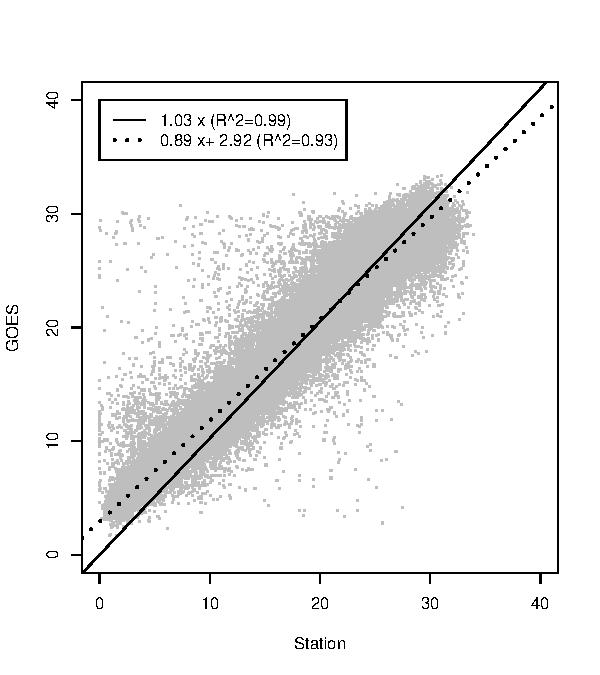
\includegraphics{Rs_R.pdf}
  \caption{ A comparison of measured vs. \ac{GOES} estimated
    radiation, for all \ac{CIMIS} stations over about 3 years.  }
  \label{fig:Rs}
\end{figure}

The spatial distribution of errors for \ac{Rs} is not equal over all
parts of California as shown in Figure~\ref{fig:errRns}.  The error is
reported as the root mean squared error between the measurements and
predictions.  As can be seen, the areas along the coastline and some
desert regions have the largest errors.  Most of California shows
significantly less difference between measured and predicted \ac{Rs}.

\begin{figure}[htbp]
  \centering
% This needs to become a grass file
  \resizebox{0.5\textwidth}{!}{\begin{picture}(0,0)%
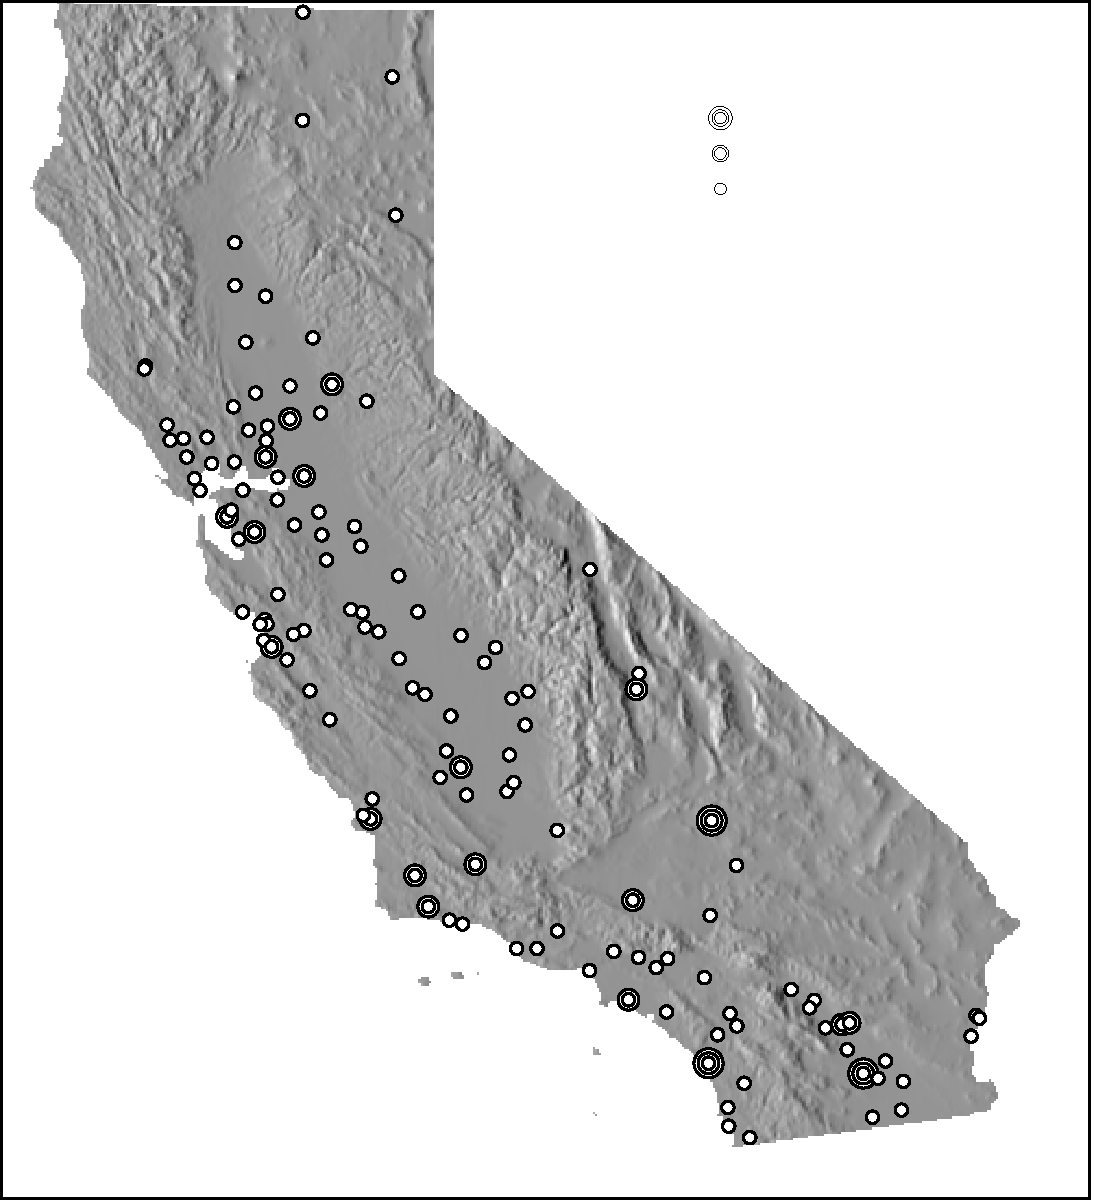
\includegraphics{figs/rms_fig.pdf}%
\end{picture}%
\setlength{\unitlength}{4144sp}%
%
\begingroup\makeatletter\ifx\SetFigFont\undefined%
\gdef\SetFigFont#1#2#3#4#5{%
  \reset@font\fontsize{#1}{#2pt}%
  \fontfamily{#3}\fontseries{#4}\fontshape{#5}%
  \selectfont}%
\fi\endgroup%
\begin{picture}(8319,9144)(1666,-9205)
\put(6031,-601){\makebox(0,0)[lb]{\smash{{\SetFigFont{14}{16.8}{\rmdefault}{\mddefault}{\updefault}{\color[rgb]{0,0,0}Average RMS Errors}%
}}}}
\put(7336,-1051){\makebox(0,0)[lb]{\smash{{\SetFigFont{14}{16.8}{\rmdefault}{\mddefault}{\updefault}{\color[rgb]{0,0,0}$> 0.2$}%
}}}}
\put(6436,-1321){\makebox(0,0)[lb]{\smash{{\SetFigFont{14}{16.8}{\rmdefault}{\mddefault}{\updefault}{\color[rgb]{0,0,0}$0.2 >$}%
}}}}
\put(7336,-1276){\makebox(0,0)[lb]{\smash{{\SetFigFont{14}{16.8}{\rmdefault}{\mddefault}{\updefault}{\color[rgb]{0,0,0}$> 0.1$}%
}}}}
\put(6436,-1591){\makebox(0,0)[lb]{\smash{{\SetFigFont{14}{16.8}{\rmdefault}{\mddefault}{\updefault}{\color[rgb]{0,0,0}$0.1 >$}%
}}}}
\end{picture}%
}
  \label{fig:errRns}
  \caption{
%
    Percent difference between the \ac{CIMIS}
    measurements and \ac{GOES} estimations of \ac{Rs} for California.
%
  }
\end{figure}

\subsubsection{Net Longwave Radiation, \ac{Rnl}}
\label{sec:rnl}

The daily net longwave radiation, \ac{Rnl}, is derived from the
Stefan-Boltzmann law, with an estimation of the net emissivity based
on water vapor.

\begin{equation}
   \ac{Rnl} = -(1.35K-0.35)(0.34-0.14\sqrt{e_a})\sigma\frac{(T_x+273.16)^4+(T_n+273.16)^4}{2}
\end{equation}

Most of these values are based on interpolated values with the
exception of \ac{K}.  \ac{CIMIS} estimates cloud cover as a ratio
between the measured solar radiation and predicted clear sky
radiation; similar to the clear sky factor described in
Section~\ref{sec:cloud-brightn-clear}, but with a different clear sky
radiation model.  Figure~\ref{fig:Rlw} shows the difference between
\ac{CIMIS} \ac{Rnl} and \ac{Rnl} using \ac{GOES} estimated \ac{K}
factors.  As in the \ac{Rs} comparison, the \ac{GOES} method
over-predicts \ac{Rnl} in the cloudy regions and under-predicts in the
clear regions.  Why this is more pronounced in the \ac{Rnl} comparison
might be because of the difference in the calculation of the cloud
factor, \ac{K}.  Since clear sky radiation is not a measured value at
the \ac{CIMIS} stations, it is unclear which estimation is more
accurate.
        
\begin{figure}[htbp]
  \centering
  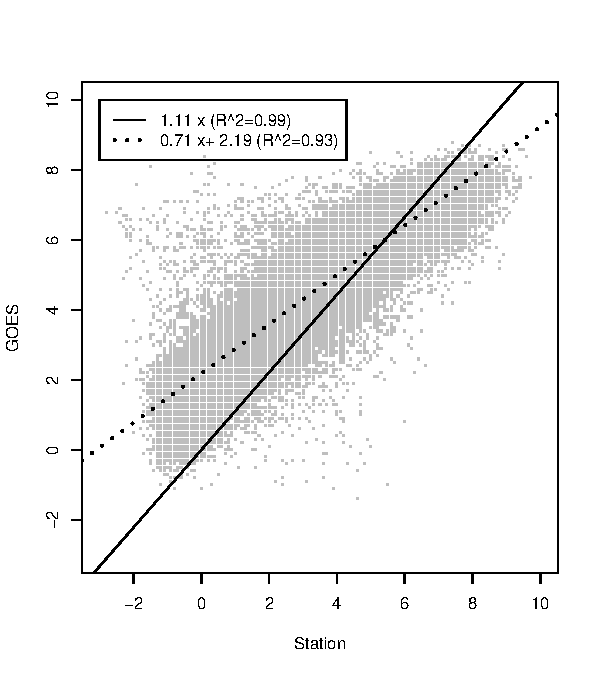
\includegraphics{Rnl_R.pdf}
  \caption{
%
    \ac{GOES} based estimates of \acl{Rnl} compared to \ac{CIMIS}
    ground station estimates.
%
  }
  \label{fig:Rlw}
%\vspace*{12pt}\hrule
\end{figure}

\subsection{Winter Net Radiation Estimation Problems}

Two winter phenomena in California adversely affected the
net radiation predictions on certain occasions.  These phenomena
are snowfall and persistent fog, both common occurrences in
California.  Both problems lead to inaccurate estimations of surface
albedo, which lead to inaccurate estimations of cloud cover, which
lead to inaccurate estimations of net radiation.  In the case of
snowfall, the current method compares snowfall to the previous albedo
and perceives freshly fallen snow as cloud cover, resulting in over
predicting clouds and under predicting net radiation.  In the case of
persistent fog, a 14 day region of continuous fog will cause a large
over prediction of albedo, and subsequently will under predict cloud
cover and over predict net radiation for cloud covered regions.

A modification to the existing model, including adding additional
\ac{GOES} imager channels to differentiate between cloud and snow, and
fog and surface is being planned.

\section{Measurement Uncertainty}
\label{sec:meas-uncert}

The \ac{ET0} model provides a single \ac{ET0} value per pixel.  To
support the use the output it is necessary to provide some information
about the reliability of the predictions.  For our model,
interpolated data presents problems of under sampling and poorly
distributed weather stations, while satellite imagery presents
problems with the method of retrieval and derivation used.

To estimate uncertainty, Monte Carlo simulations are run on the daily
estimations.  Normally distributed errors are associated with each
input parameter to the \ac{ET0} calculation, for each pixel in the
image.  Because of the proximity of \ac{CIMIS} stations, elevation
differences, and other spatially varying considerations, the errors
for each parameter vary across the image.  Table~\ref{tab:errors}
summarizes the standard deviation used for each parameter.  Here, the
difference of the two estimations for temperatures are used to
set error bounds on \ac{Tn}, \ac{Tx}, \ac{dewp}, and,
indirectly, \ac{ea} and \ac{es}.  The radiation parameter errors are
modeled as percentages of the radiation values.  \ac{Rs}, especially,
has a higher error than the comparison to the \ac{CIMIS} data suggest,
but was increased to simulate differences in calculations of \ac{Rso}
as mentioned in Section~\ref{sec:radiation}.  Wind speed, \ac{U2},
errors were estimated.

\begin{table}
  \centering
  \caption{Error contributions}
  \begin{tabular}{l|c|l}
    Parameter & Std. Dev. & Description \\
    \hline \hline
    \ac{Tx} & $\sqrt{2}|\Delta(\ac{Tx})|$ & $\Delta(\ac{Tx})$ is difference in interpolations \\
    \ac{Tn} & $\sqrt{2}|\Delta(\ac{Tn})|$ & $\Delta(\ac{Tn})$ is difference in interpolations \\
    \ac{dewp} & $\sqrt{2}|\Delta(\ac{dewp})|$ & $\Delta(\ac{dewp})$ is difference in interpolations \\
    \ac{ea} & $\sqrt{2}|\Delta(\ac{es})|$ & $\Delta(\ac{ea})$ is difference in interpolations \\
    \ac{Rs} & 0.15*\ac{Rs} & Estimated from different \ac{Rs} calculations \\
    \ac{Rnl} & 0.15*\ac{Rnl} & Estimated from different \ac{Rnl} calculations \\
    \ac{U2} & 0.25*\ac{U2} & Estimated \\
  \end{tabular}
  \label{tab:errors}
\end{table}

For each day, standard deviation maps are computed for every
parameter.  For each parameter, an image of random Gaussian
distributed errors with mean 0 and standard deviation 1 is calculated
and multiplied with the parameter's standard deviation map.  The
resultant errors are added to the estimated values for each parameter,
and \ac{ET0} is calculated.  This is carried out for a number of error
maps.  The variance of the calculated \ac{ET0} estimations can then be
used as an estimate to the error associated with the \ac{ET0}
prediction.

Because of computing limitations, only 10 separate Monte-Carlo runs
are performed per day.  This number is low enough that the resultant
maps of predicted error in the \ac{ET0} calculations shows
randomization patterns and are speckled.  To improve the output, the
error map is run through a 3x3 averaging filter.  In a sense, this
creates a pseudo error map of 90 Monte-Carlo runs, and eliminates the
random patterns.

Figure~\ref{fig:error-map} shows the average error estimates of
uncertainty for \ac{ET0} as isolines on the average \ac{ET0} values.
This is for the month of August, 2005.

\begin{figure}
  \centering
  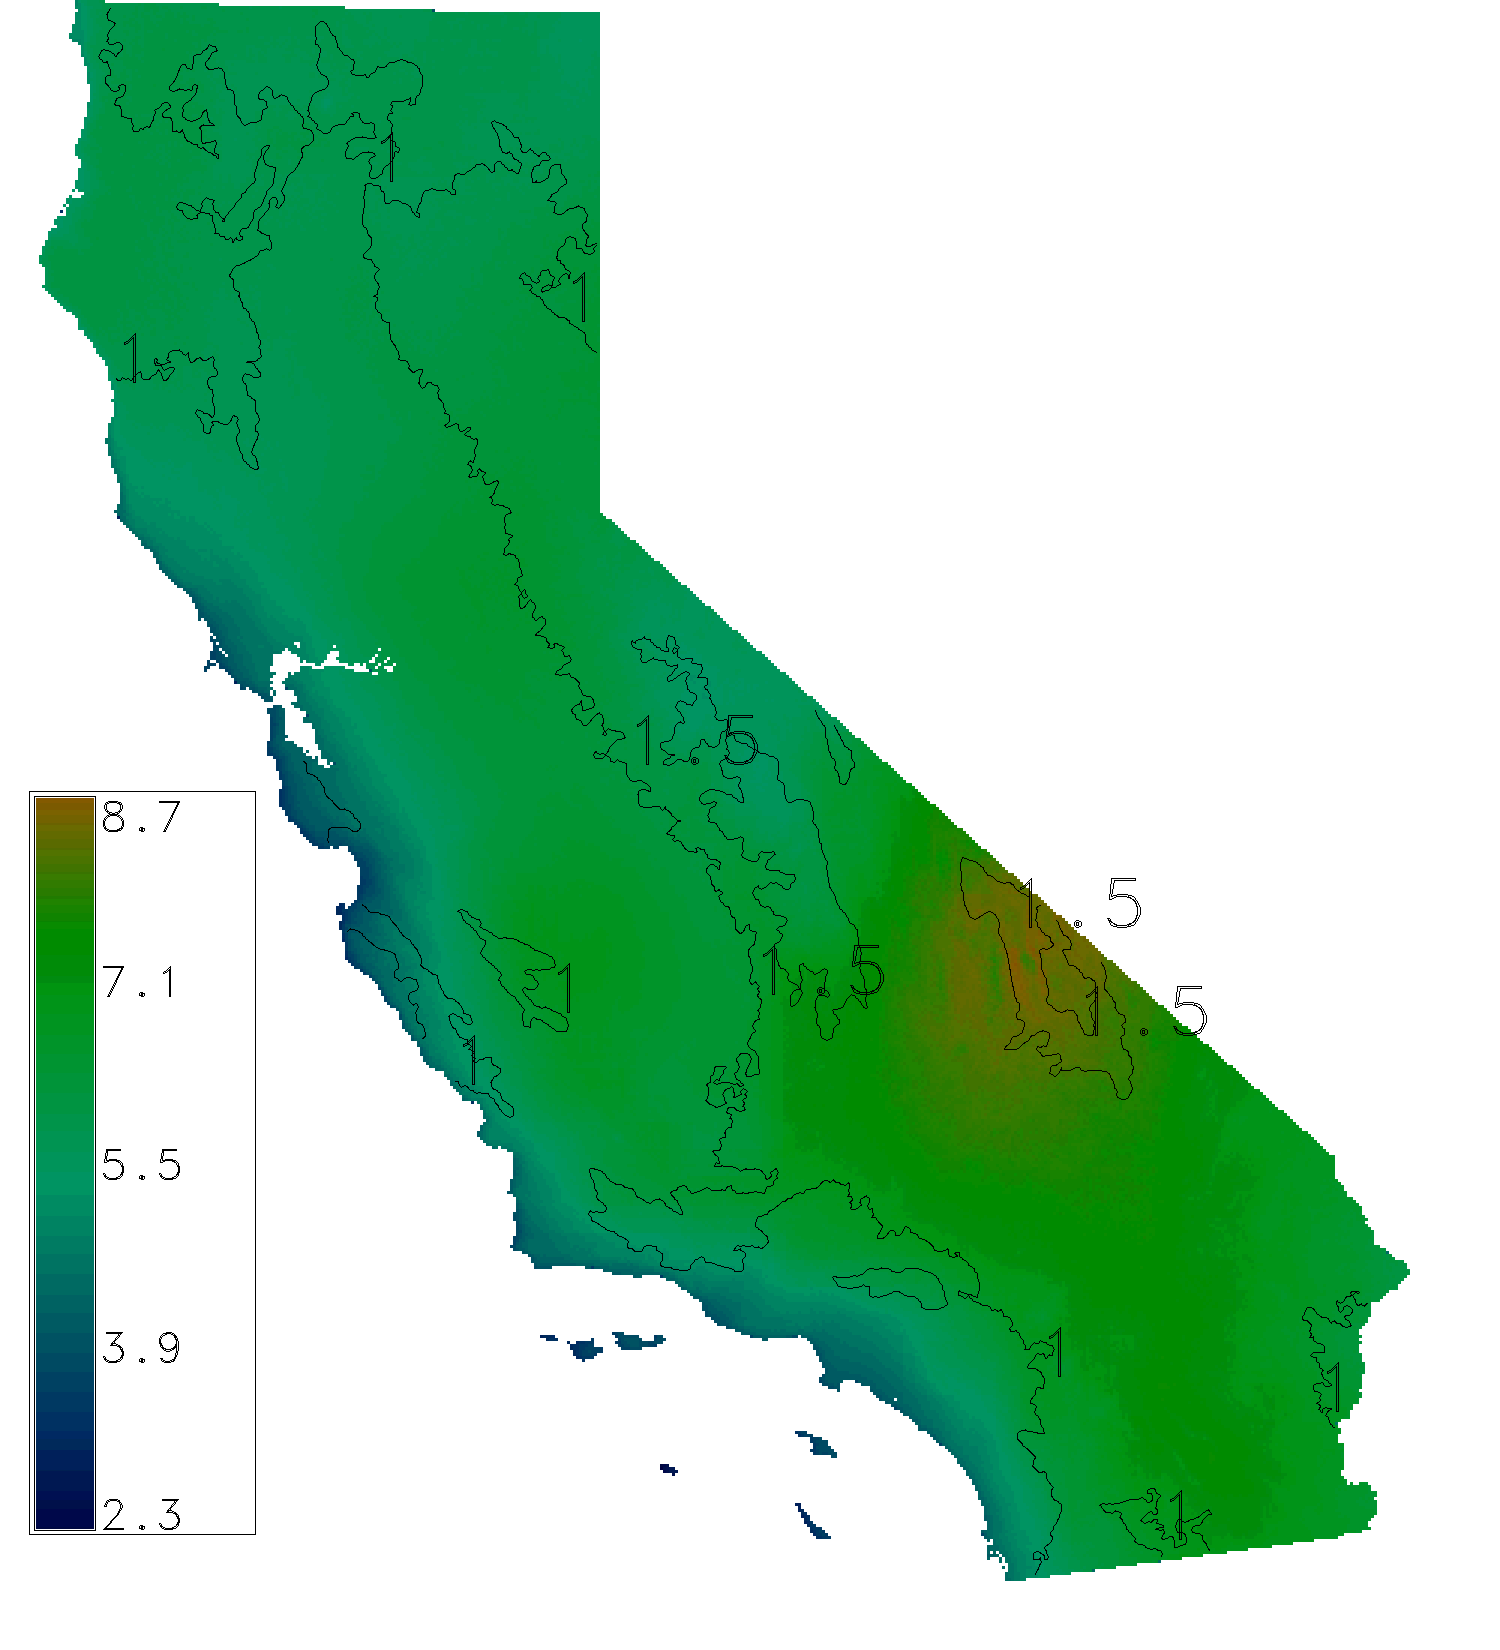
\includegraphics[width=.5\textwidth]{figs/errors-2005-08.png}
  \caption{Estimated \ac{ET0} error for 2005-08.  Raster colors indicate estimated \ac{ET0}, and isolines show error estimates with labels in \unit{mm}.}
  \label{fig:error-map}
\end{figure}

Uncertainty analysis is run every day to estimate spatial uncertainty
of the results.  However, these estimates can be misleading in
certain cases, for example, the error estimation for the temperature
parameters assumes there is no bias in the two interpolation methods.
This has not been validated.

% \section{Average \ac{ET0} values}

% Although the main goal of producing daily \ac{ET0} maps is to provide
% support for short term irrigation strategies, examination of long term
% averages can provide insight into major \ac{ET} regimes in California,
% and provide validation of the model when compared to similar maps.
% Approximately 3 years of data for each month were combined to provide
% 12 monthly averages of \ac{ET0} throughout California.  A \ac{PCA}
% transformation~\citep{richards86remot-sensin} was applied to these 12
% values, and the top three components were used in an unsupervised
% classification of California's \ac{ET0} zones.
% Figure~\ref{fig:pca_graph} shows the contributions of the monthly
% \ac{ET0} values to each \ac{PCA} vector.  These components can be
% roughly identified as picking out the total yearly amount of \ac{ET0}
% for a pixel and the spring and summer contributions to the \ac{ET0}.

% \begin{figure}
%   \centering
%   \begin{picture}(0,0)%
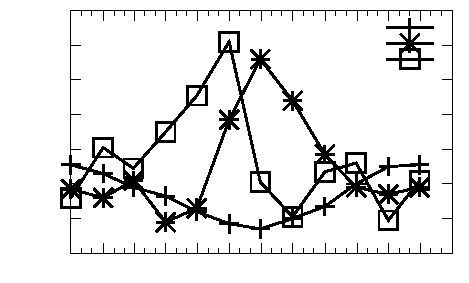
\includegraphics{monthly/pca_fig.pdf}%
\end{picture}%
\setlength{\unitlength}{3947sp}%
%
\begingroup\makeatletter\ifx\SetFigFont\undefined%
\gdef\SetFigFont#1#2#3#4#5{%
  \reset@font\fontsize{#1}{#2pt}%
  \fontfamily{#3}\fontseries{#4}\fontshape{#5}%
  \selectfont}%
\fi\endgroup%
\begin{picture}(3747,2257)(1271,-3950)
\put(1763,-3773){\makebox(0,0)[rb]{\smash{{\SetFigFont{10}{12.0}{\familydefault}{\mddefault}{\updefault}-0.6}}}}
\put(1763,-3496){\makebox(0,0)[rb]{\smash{{\SetFigFont{10}{12.0}{\familydefault}{\mddefault}{\updefault}-0.4}}}}
\put(1763,-3219){\makebox(0,0)[rb]{\smash{{\SetFigFont{10}{12.0}{\familydefault}{\mddefault}{\updefault}-0.2}}}}
\put(1763,-2942){\makebox(0,0)[rb]{\smash{{\SetFigFont{10}{12.0}{\familydefault}{\mddefault}{\updefault} 0}}}}
\put(1763,-2664){\makebox(0,0)[rb]{\smash{{\SetFigFont{10}{12.0}{\familydefault}{\mddefault}{\updefault} 0.2}}}}
\put(1763,-2387){\makebox(0,0)[rb]{\smash{{\SetFigFont{10}{12.0}{\familydefault}{\mddefault}{\updefault} 0.4}}}}
\put(1763,-2110){\makebox(0,0)[rb]{\smash{{\SetFigFont{10}{12.0}{\familydefault}{\mddefault}{\updefault} 0.6}}}}
\put(1763,-1833){\makebox(0,0)[rb]{\smash{{\SetFigFont{10}{12.0}{\familydefault}{\mddefault}{\updefault} 0.8}}}}
\put(1838,-3898){\makebox(0,0)[b]{\smash{{\SetFigFont{10}{12.0}{\familydefault}{\mddefault}{\updefault}Jan}}}}
\put(2100,-3898){\makebox(0,0)[b]{\smash{{\SetFigFont{10}{12.0}{\familydefault}{\mddefault}{\updefault}Feb}}}}
\put(2345,-3898){\makebox(0,0)[b]{\smash{{\SetFigFont{10}{12.0}{\familydefault}{\mddefault}{\updefault}Mar}}}}
\put(2598,-3898){\makebox(0,0)[b]{\smash{{\SetFigFont{10}{12.0}{\familydefault}{\mddefault}{\updefault}Apr}}}}
\put(2852,-3898){\makebox(0,0)[b]{\smash{{\SetFigFont{10}{12.0}{\familydefault}{\mddefault}{\updefault}May}}}}
\put(3105,-3898){\makebox(0,0)[b]{\smash{{\SetFigFont{10}{12.0}{\familydefault}{\mddefault}{\updefault}Jun}}}}
\put(3359,-3898){\makebox(0,0)[b]{\smash{{\SetFigFont{10}{12.0}{\familydefault}{\mddefault}{\updefault}Jul}}}}
\put(3612,-3898){\makebox(0,0)[b]{\smash{{\SetFigFont{10}{12.0}{\familydefault}{\mddefault}{\updefault}Aug}}}}
\put(3874,-3898){\makebox(0,0)[b]{\smash{{\SetFigFont{10}{12.0}{\familydefault}{\mddefault}{\updefault}Sep}}}}
\put(4127,-3898){\makebox(0,0)[b]{\smash{{\SetFigFont{10}{12.0}{\familydefault}{\mddefault}{\updefault}Oct}}}}
\put(4381,-3898){\makebox(0,0)[b]{\smash{{\SetFigFont{10}{12.0}{\familydefault}{\mddefault}{\updefault}Nov}}}}
\put(4634,-3898){\makebox(0,0)[b]{\smash{{\SetFigFont{10}{12.0}{\familydefault}{\mddefault}{\updefault}Dec}}}}
\put(4888,-3898){\makebox(0,0)[b]{\smash{{\SetFigFont{10}{12.0}{\familydefault}{\mddefault}{\updefault}Jan}}}}
\put(1387,-2741){\rotatebox{90.0}{\makebox(0,0)[b]{\smash{{\SetFigFont{10}{12.0}{\familydefault}{\mddefault}{\updefault}Weight}}}}}
\put(4288,-1970){\makebox(0,0)[rb]{\smash{{\SetFigFont{10}{12.0}{\familydefault}{\mddefault}{\updefault}PC1: Yearly Total}}}}
\put(4288,-2095){\makebox(0,0)[rb]{\smash{{\SetFigFont{10}{12.0}{\familydefault}{\mddefault}{\updefault}PC2: Summer Values}}}}
\put(4288,-2220){\makebox(0,0)[rb]{\smash{{\SetFigFont{10}{12.0}{\familydefault}{\mddefault}{\updefault}PC3: Spring Values}}}}
\end{picture}%

%   \caption{Three most important principle
%     component vectors for monthly contribution to \ac{ET0}}
% \label{fig:pca_graph}
% \end{figure}

% An unsupervised classification of 6 regions derived from these
% \ac{PCA} vectors is shown in Figure~\ref{fig:et0-classes}.  These are
% generally labeled with their prominent location within California.
% Given these regions, summary information about expected \ac{ET0}
% amounts through the year can be calculated.  These are shown in
% Table~\ref{tab:et0-classes}, which describes the average \ac{ET0} for
% each region and month.

% \begin{figure}
%   \centering
%   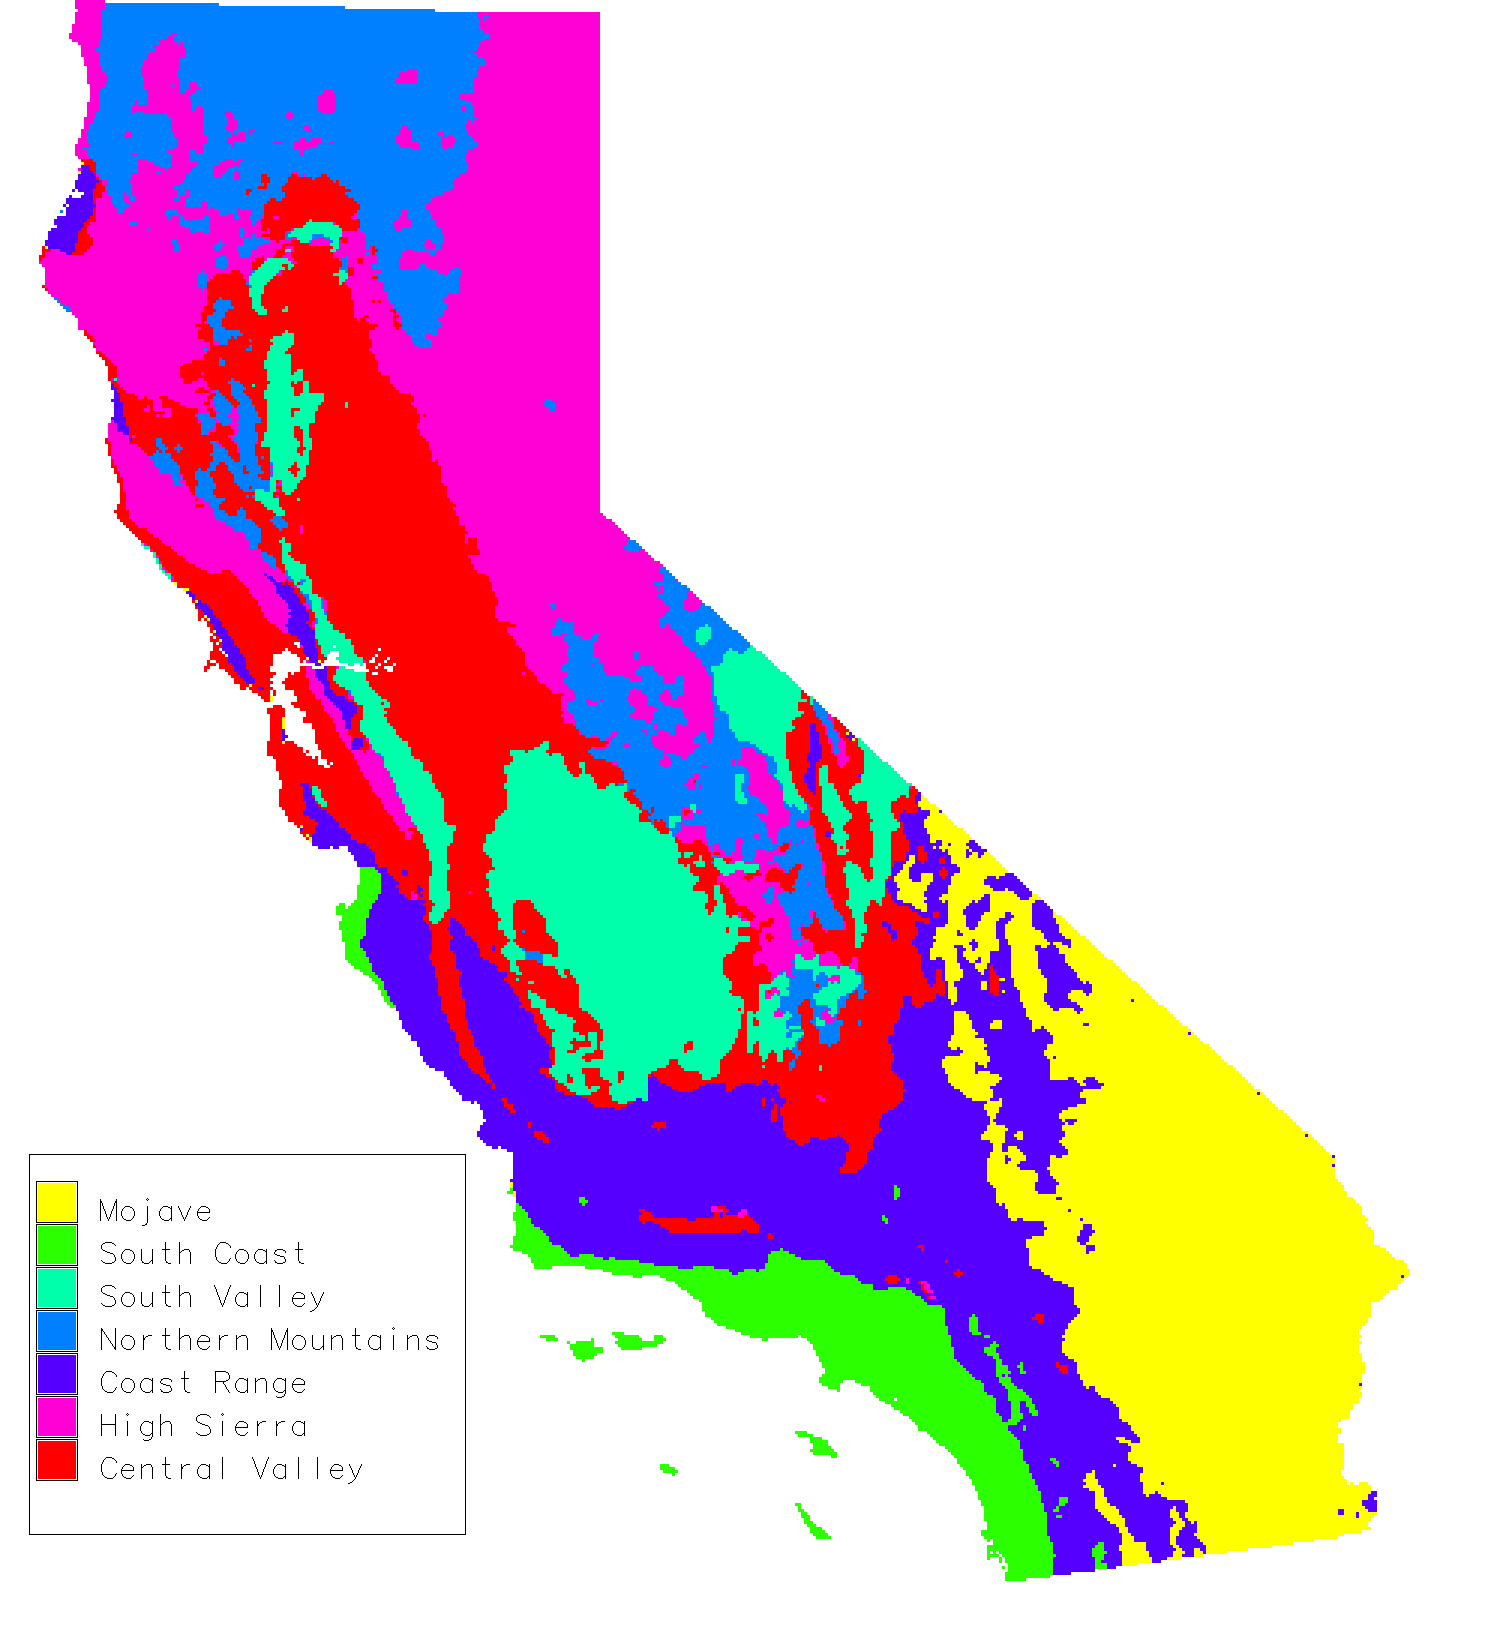
\includegraphics[width=.5\textwidth]{monthly/classes.png}  
%   \caption{Unsupervised classification \ac{ET0} regions based on three
%     years of data.}
%   \label{fig:et0-classes}
% \end{figure}

% \begin{table}
%   \centering
%   \caption{Average \ac{ET0} values for different California regions}
%   \begin{tabular}{c|c|c|c|c|c|c|c}
% & South & South & Northern & Mojave & Coast & High & Central \\
% Month & Coast & Valley & Mountains & Desert & Range & Sierra & Valley \\
% \hline \hline
% Jan & 1.68 & 0.88 & 0.73 & 2.01 & 1.47 & 0.75 & 0.88 \\
% Feb & 2.13 & 1.68 & 1.46 & 2.69 & 2.11 & 1.47 & 1.69 \\
% Mar & 3.01 & 2.93 & 2.54 & 4.38 & 3.35 & 2.61 & 2.88 \\
% Apr & 3.60 & 3.85 & 2.93 & 5.57 & 4.15 & 2.99 & 3.61 \\
% May & 4.40 & 5.28 & 4.23 & 7.22 & 5.49 & 4.26 & 4.90 \\
% Jun & 4.52 & 6.47 & 5.78 & 8.25 & 6.40 & 5.65 & 6.06 \\
% Jul & 5.33 & 6.87 & 6.50 & 8.21 & 6.90 & 6.51 & 6.48 \\
% Aug & 4.94 & 6.05 & 5.47 & 7.20 & 6.22 & 5.55 & 5.73 \\
% Sep & 4.10 & 4.78 & 4.20 & 6.20 & 5.09 & 4.29 & 4.65 \\
% Oct & 2.62 & 2.76 & 2.35 & 3.86 & 3.13 & 2.42 & 2.77 \\
% Nov & 1.98 & 1.36 & 1.04 & 2.24 & 1.86 & 1.08 & 1.33 \\
% Dec & 1.54 & 0.88 & 0.68 & 1.80 & 1.40 & 0.70 & 0.86 \\    
%   \end{tabular}
%   \label{tab:et0-classes}
% \end{table}

% The Department of Water Resources and UC Davis, have previously
% developed a map of \ac{ET0} zones in
% California~\citep{cimis99calif-refer}, shown in Figure~\ref{fig:et0}.
% This map was the result of experts delineating regions in California,
% based on long term weather station data.  Comparison of this map to
% that of Figure~\ref{fig:et0-classes} show good agreement, and provide
% a qualitative validation of the \ac{GOES} and \ac{CIMIS} derived map
% products.

% \begin{figure}[htbp]
%   \centering
%   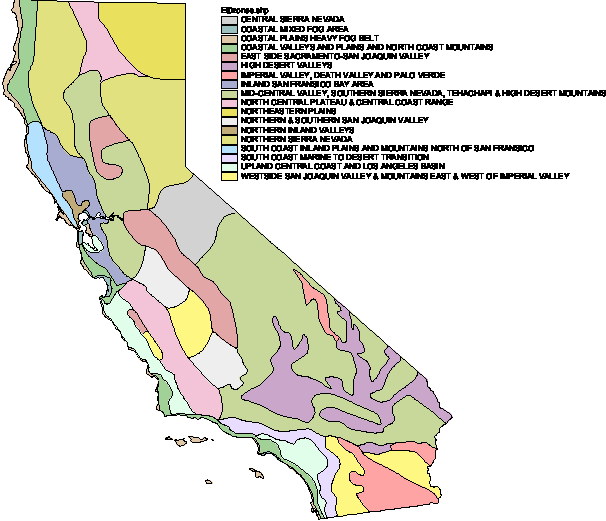
\includegraphics[width=0.5\textwidth]{etomap_simple.pdf}
%   \caption{%
%     Map of different \ac{ET0} zones for California.  18 separate
%     zones, derived from monthly \ac{ET0} averages, delineate different
%     regions and influences in California. }
%   \label{fig:et0}
% %\vspace*{12pt}\hrule
% \end{figure}


\section{Conclusions}

\ac{ET} is an important indicator in both agricultural and urban
settings and can address water needs for a variety of water issues,
such as irrigation scheduling.

We have demonstrated a method of creating daily \ac{ET0} maps
for California using satellite and ground station data.  The current
method provides good estimates of \ac{ET0} and will be incorporated in
the \acl{CIMIS} program, providing users access to spatial
distributions of \ac{ET0}.  The model has been used with \ac{GOES} and
\ac{CIMIS} data for approximately three years, since February, 2003.

Net radiation models combined with \ac{GOES} estimates of cloud cover
is an effective method of obtaining spatial estimations of solar
radiation.  Some events like snowfall and persistent fog, lead to
erroneous cloud cover predictions.  Including additional \ac{GOES}
channels to detect these events is an important next step.

Variations in the temperature distributions throughout California are
caused by multiple forces and can be difficult to model completely
with interpolation methods alone, especially in regions where stations
are sparse.  One possibility being investigated will use weather
prediction models, run at small time scales, and periodically modified
by near real-time hourly data from weather stations to more accurately
model the spatial variability of surface parameters.

Monte-Carlo methods can be used on spatial calculations to understand
more accurately what the impact of uncertainties in parameter
estimations can have on final model outputs.


\bibliographystyle{elsart-harv}
\bibliography{../cimis}

\end{document}


% LocalWords:  evapotranspiration albedo irradiance imager snowpack snowmelt streamflow CIMIS FAO
% LocalWords:  stomata micrometeorological Monteith emissitivity Linke isolines
% LocalWords:  psychrometric Heliosat turbidity sigmoidal longwave DayMet